\documentclass[oneside, a4paper, spanish, links]{amca}
\usepackage[spanish]{babel}
\usepackage{graphicx}
\usepackage{amsmath, amsfonts}
\usepackage{subcaption}
\usepackage{mwe}
\usepackage{listings}

\usepackage[section]{placeins}

\usepackage{float}

\usepackage[utf8]{inputenc}

\usepackage[backend=biber]{biblatex} %paquete

\pagestyle{plain}
\pagenumbering{arabic}


\addbibresource{biblioteca.bib}        %El paquete para la bilbiografía

\title{ANÁLISIS DE VIBRACIONES DE AUTOMÓVIL COMO SISTEMA DE 4 GRADOS DE LIBERTAD CON SIMETRÍA LONGITUDINAL}


\author[\voidaffil]{Gino Avanzini}
\author[\voidaffil]{Emiliano Cabrino}
\author[\voidaffil]{Agustín Lezcano}


\affil[\voidaffil]{Mecánica Vibratoria, 
Facultad de Ingeniería, 
Universidad Nacional de Cuyo}


\begin{document}
\vspace{3cm}

\maketitle
\begin{keywords}
Análisis de vibraciones, MATLAB.
\end{keywords}


\section{Introducción}
En este trabajo se propone el análisis de vibraciones de un vehículo de cuatro ruedas ante cargas externas armónicas y ante cargas impulsivas. En la primera parte se deriva el modelo matemático a partir del modelo físico, el cual es una simplificación de un automóvil de 4 ruedas. Realizando un análisis de autovalores y autovectores encontraremos los modos y frecuencias naturales de vibración. Luego calculamos la respuesta del sistema en vibraciones libres y la respuesta ante una carga armónica, la cual está inspirada en el ``serrucho`` que se observa en algunos caminos de tierra. Por último analizamos la respuesta ante una carga impulsiva. 

Para la realización de este trabajo no se observará un modelo experimental sino que se realizará un modelo numérico de un vehículo de 4 GDL, partiendo del supuesto de simetría longitudinal. La rigidez existente entre el suelo y el vehículo será modelada mediante resortes y el sistema de amortiguamiento del vehículo propiamente dicho será modelado por un resorte y un amortiguador. Se tendrá en cuenta el cabeceo o \textit{pitch}.

\newpage
\section{Modelado y métodos numéricos}
\subsection{Modelo físico}

Nuestro problema implica modelar un automóvil de cuatro ruedas y obtener la respuesta del mismo ante distintas excitaciones. El sistema puede ser modelado con simetría longitudinal, por lo cual se supone respuestas idénticas a cada lado del vehículo y tenemos en cuenta los movimientos independientes de las zonas delantera y trasera del automóvil. Como modelo utilizaremos un sistema de 4 grados de libertad, siendo estos los movimientos verticales de las ruedas, la rotación alrededor del centro de masa del chasis (cabeceo o \textit{pitch}) y el movimiento vertical del chasis (ver Figura \ref{fig: modelo}).

\begin{figure}[ht] %lo que va entre corchetes es donde lo quiero poner
    \centering
    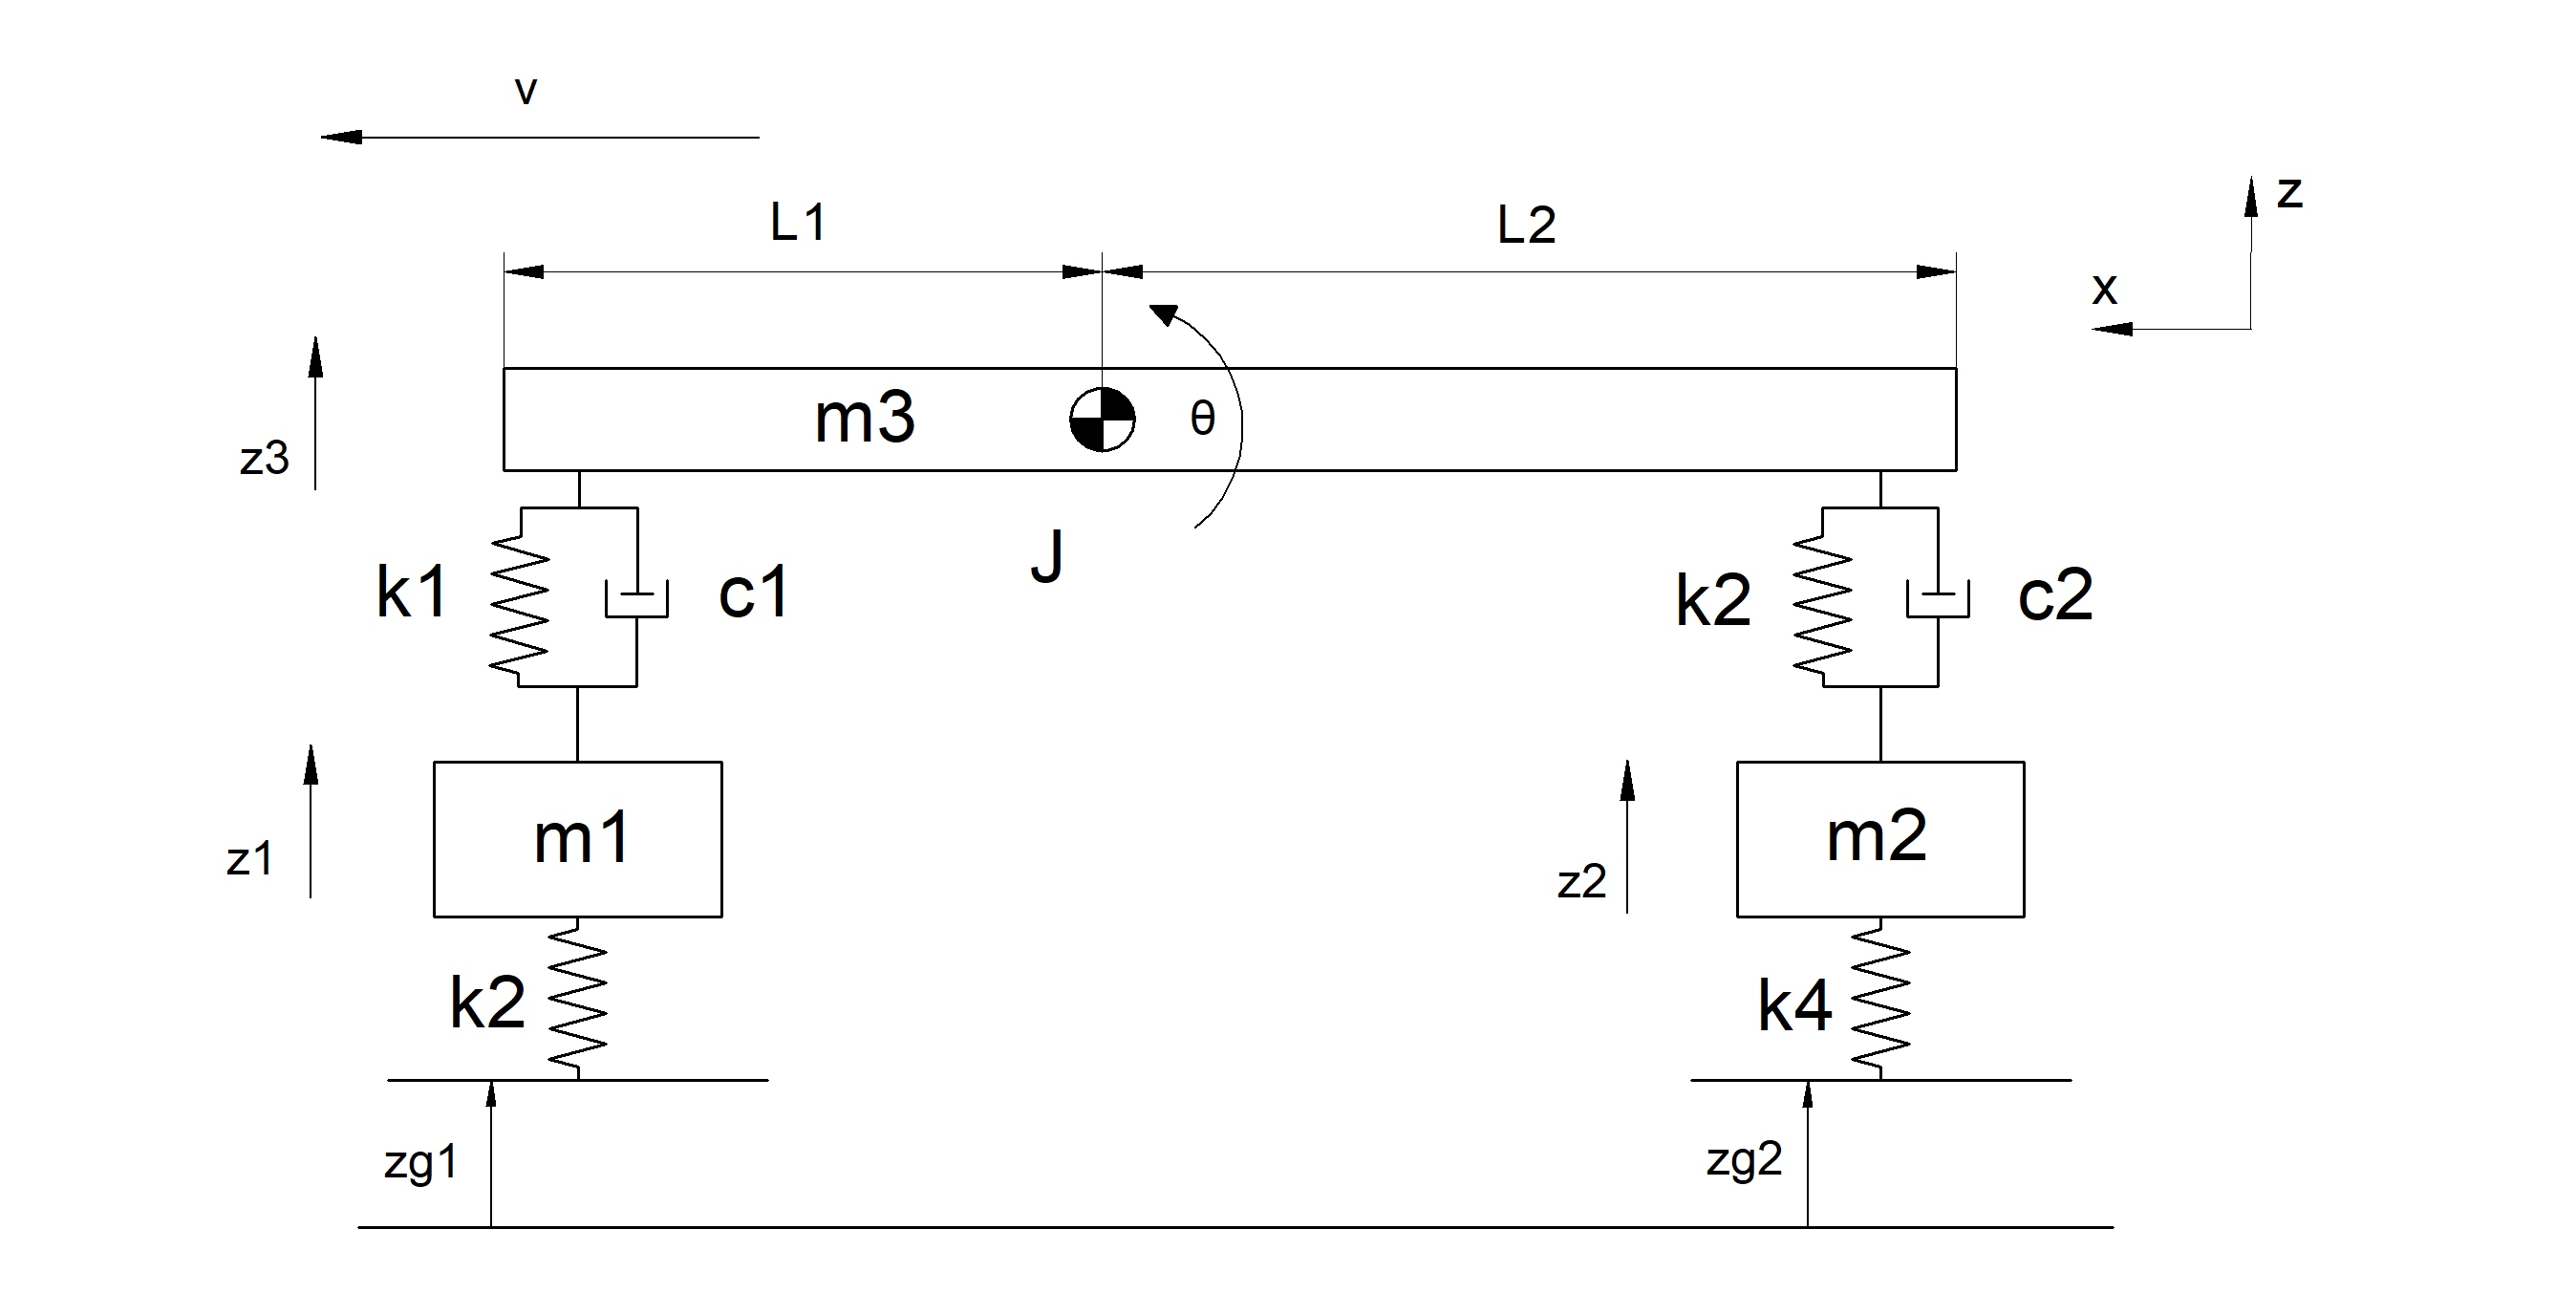
\includegraphics[width=1
    \textwidth]{modelo.png}
    \caption{Modelo utilizado}
    \label{fig: modelo} % es un tag de la imagen
\end{figure}

Como parámetros del sistema se tienen la rigidez suelo-rueda (cubierta) y los parámetros k y c del sistema de amortiguamiento del vehículo. Además se considera la masa del conjunto rueda-cubierta y el momento de inercia y la masa del chasis. Los valores de la rigidez en la parte delantera y trasera del vehículo son distintos debido a que la masa no está distribuida de manera simétrica.
En el caso en estudio se analizará la dinámica vertical, que está relacionada con el comportamiento del vehículo cuando es sometido a excitaciones de base, las cuales pueden ser irregularidades del suelo (nuestro caso de estudio). 

Para el análisis de las cargas se usó el análisis de movimiento del soporte. De esta manera los grados de libertad $z_1$ y $z_2$ son absolutos, es decir, están referenciados a la línea de cero de la carga aplicada. Las cargas en sí son desplazamientos de los soportes los cuales están acoplados a $z_1$ y $z_2$ mediante las rigideces \textit{$k_2$} y \textit{$k_4$}.

\subsection{Modelo matemático}

Se definen los grados de libertad y los movimientos de la base como:

\begin{equation}
    Z=(z_1, z_2, z_3, \theta)
\end{equation}
\begin{equation}
    Z_g=(zg_1, zg_2, 0, 0)
\end{equation}

Luego de determinar los grados de libertad y movimientos de la base, se utiliza el método de Lagrange para encontrar el sistema de ecuaciones diferenciales acopladas. El lagrangiano es $L=T-V$ siendo $T$ la energía cinética y $V$ la potencial y, teniendo en cuenta las energías no conservativas ($D$), se pueden encontrar las ecuaciones diferenciales de cada grado de libertad a partir de la ecuación de Lagrange:

\begin{equation}
\frac{d}{dt}(\frac{\partial{T}}{\partial{\dot{x}_i}})-(\frac{\partial{T}}{\partial{x_i}})+(\frac{\partial{V}}{\partial{\dot{x}_i}})+(\frac{\partial{D}}{\partial{\dot{x}_i}})=0
\label{ec: Lagrange}
\end{equation}

Aplicando (\ref{ec: Lagrange}) a cada uno de los grados de libertad queda definido el sistema de ecuaciones diferenciales, en forma matricial:

\begin{equation}
    M\Ddot{Z}+C\dot{Z}+KZ=LZ_g
    \label{eq: ec matricial}
\end{equation}

Con las siguientes matrices: 

$M=$
\begin{bmatrix}             %matriz de masas
{m_1} & {0} & {0} & {0} \\ 
{0} & {m_2} & {0} & {0} \\
{0} & {0} & {m_3} & {0} \\
{0} & {0} & {0} & {J}
\end{bmatrix}

$C=$
\begin{bmatrix}             %matriz C
{c_1} & {0} & {-c_1} & {-c_1*L_1} \\
{0} & {c_2} & {-c_2} & {c_2*L_2} \\
{-c_1} & {-c_2} & {c_1 + c_2} & {c_1*L_1-c_2*L_2} \\
{-c_1*L_1} & {c_2*L_2} & {c_1*L_1} & {c_1*L_1^2 + c_2*L_2^2}
\end{bmatrix}

$K=$
\begin{bmatrix}             %matriz K
{k_1+k_2} & {0} & {-k_1} & {-k_1*L_1}\\
{0} & {k_3+k_4} & {-k_3} & {-k_3*L_2}\\
{-k_1} & {-k_3} & {k_1+k_3} & {k_1*L_1-k_3*L_2}\\
{-k_1*L_1} & {k_3*L_2} & {k_1*L_1-k_3*L_2} & {k_1*L_1^2+k_3*L_2^2}
\end{bmatrix}

    $\Ddot{Z}=$
\begin{bmatrix}             %vector de aceleración
{\Ddot{z_1}}\\
{\Ddot{z_2}}\\
{\Ddot{z_3}}\\
{\Ddot{\theta}}
\end{bmatrix}
$\dot{Z}=$
\begin{bmatrix}             %vector de velocidad
{\dot{z_1}}\\{\dot{z_2}}\\{\dot{z_3}}\\{\dot{\theta}}
\end{bmatrix}
$Z=$
\begin{bmatrix}             %vector de posición
{{z_1}}\\{{z_2}}\\{{z_3}}\\{{\theta}}
\end{bmatrix}

$L=$
\begin{bmatrix}             %matriz de participación de carga
{k2}&{0}&{0}&{0}\\{0}&{k4}&{0}&{0}\\{0}&{0}&{0}&{0}\\{0}&{0}&{0}&{0}
\end{bmatrix} 
$Z_g=$
\begin{bmatrix}             %vector de posición relativa al suelo
{zg_1}\\{zg_2}\\{0}\\{0}
\end{bmatrix}

\\
Los parámetros utilizados junto con sus valores son los que se encuentran en la tabla \ref{tab: parametros}. Para la elaboración de la tabla se han considerado valores numéricos para los parámetros, los cuales fueron incluidos tomando como referencia los valores obtenidos en Tica Mihai\ref{libro_tabla}.

\begin{table}[h]
\begin{tabular}{|l|l|l|}
\hline
\textbf{Parámetro}                                       & \textbf{Símbolo} & \textbf{Valor}                \\ \hline
Masas de las ruedas                                      & $m_1 = m_2$          & 50 kg                       \\ \hline
Masa del chasis                                          & $m_3$                & 1000 kg                     \\ \hline
Rigidez de la suspensión delantera                       & $k_1$                & 80000 N/m                   \\ \hline
Rigideces de las cubiertas                               & $k_2 = k_4$          & 300000 N/m                  \\ \hline
Rigidez de la suspensión trasera                         & $k_3$                & 60000 N/m                   \\ \hline
Constante de amortiguamiento de los amortiguadores       & $c_1 = c_2$          & 4000 Ns/m                   \\ \hline
Distancia longitudinal entre el eje y la rueda delantera & $L_1$                & 1,4 m                       \\ \hline
Distancia longitudinal entre el eje y la rueda trasera   & $L_2$                & 2 m                         \\ \hline
Momento de inercia del chasis                            & $J$                  & 500 kg.m^2                 \\ \hline
\end{tabular}
\caption{Tabla de parámetros del sistema}
\label{tab: parametros}
\end{table}

Para encontrar la respuesta del sistema a las distintas excitaciones había principalmente dos acercamientos: utilizar el método de descomposición modal y encontrar las respuestas modales independientes o resolver las ecuaciones en coordenadas geométricas acopladas. Se eligió lo último porque nuestra matriz de amortiguamientos no es diagonalizable y no es posible realizar descomposición modal. 


\subsection{Métodos numéricos}

Para la resolución del sistema ecuaciones diferenciales (\ref{eq: ec matricial}) previamente planteado se utilizaron distintos métodos numéricos, dependiendo de los resultados que se quieren obtener. Entre ellos se destacan el método de diferencias finitas centrales y el uso de la función \textit{ode45} de MATLAB (el cual está basado en un método Runge Kutta de cuarto orden). Además se obtienen los autovalores y autovectores del sistema mediante el uso de la función \textit{eig}. 

\subsubsection{Método de Diferencias Finitas}
\label{sec:dif finitas}

Se utilizó el método de diferencias finitas, un método \textit{paso a paso}, el cual se basa en el uso de los valores del paso anterior para calcular los del paso actual.
En la implementación de este método se usó la aproximación central de la derivada segunda.

Para usar este método se necesita que los valores obtenidos converjan a los valores reales de la función; esto se consigue cuando $\frac{h}{T} \leq \frac{1}{\pi}$ y es mejor si esta relación es menor a 0,1. Para el paso que utilizamos, $dt = 0.0001$, y el período de la carga con mayor frecuencia, se encuentra que la solución debe converger.

El método se puede resumir de la siguiente manera: 

\begin{equation}
    x_i=\frac{h^2}{2}(M^{-1}P_0 - M^{-1}C\dot{x}_0 - M^{-1}Kx_{i-1}) + x_{i-1} + h\dot{x}_{i-1}
\end{equation}

Siendo h el paso y $P_0$ la carga externa. Hay que recordar que $M, C, K$ son matrices de 4x4 y $P_0$, $x_i$ y $\dot{x}_i$ son vectores de 4x1. La actualización de la derivada es: 

\begin{equation}
    \dot{x_i}=\frac{2}{h}(x_i-x_{i-1})-{\dot{x}_{i-1}}
\end{equation}

\subsubsection{ode45}
\label{sec:ode45}

La función ode45 de MATLAB es un \textit{solver} de sistemas de ecuaciones diferenciales ordinarias basado el método Runge Kutta de cuarto orden. Este método resuelve sistemas de ecuaciones diferenciales de primer orden. Ya que el sistema de ecuaciones diferenciales obtenido es de segundo orden, hay que hacer una reducción de orden.

A partir del sistema (\ref{eq: ec matricial}):

\begin{equation}
    M\Ddot{Z}+C\dot{Z}+KZ=LZ_g
    \nonumber
\end{equation}

Con:

\begin{equation}
    v=\dot{Z}
    \label{eq:vd=z}
\end{equation}

Si se reemplaza (\ref{eq: ec matricial}) en (\ref{eq:vd=z}) se obtiene:

\begin{equation}
    M\dot{v}+Cv+Kz=LZg
\end{equation}

Que al despejar $\dot{v}$  
\begin{equation}
    \dot{v}=M^{-1} L Z_g - M^{-1} C v- M^{-1}K z
\end{equation}

Y resolviendo, se obtiene el siguiente sistema de ecuaciones diferenciales ordinarias de primer orden:

\begin{center}
    
\begin{bmatrix} 
{\dot{z}}\\
{\dot{v}}\\
\end{bmatrix}
=\begin{bmatrix}         
{\vect{0}} & {\vect{I}} \\ 
{-M^{-1}K} & {-M^{-1}C} \\
\end{bmatrix}
\begin{bmatrix}          
{{z}}\\
{{v}}\\
\end{bmatrix}
+
\begin{bmatrix}
{$0$}\\
{$M^{-1}LZ_g$}
\end{bmatrix}

\end{center}

El cual se puede expresar como:

\begin{equation}
  \dot{y}=Ay+B  
    \label{eq:ec ode45}
\end{equation}

Cada uno de los componentes de las matrices y vectores en el sistema anterior tiene 4 componentes; el \textit{ode45} devuelve un vector de 8x1: los desplazamientos y las velocidades de cada grado de libertad. 

Además, la función \textit{ode45} requiere de una subrutina para poder calcular cada iteración. Dicha función está basada en la ecuación (\ref{eq:ec ode45}). En MATLAB se escribió:

\begin{lstlisting}
function x_forz = vibforz_geo(t, x, M, C, K, ZERO, I, L, wl, phase, amp)
    A = [ZERO, I;
        -M\K, -M\C];
    B = [zeros(4, 1);
        M\(L*[amp*sin(wl*t);
                amp*sin(wl*t - phase);
                0;
                0])];
    
    x_forz = A*x + B;
end
\end{lstlisting}

Esta subrutina será utilizada cada vez que se llame al \textit{ode45} (ver secciones \ref{sec:vib lib} y \ref{sec: vib forz}).

\newpage
\section{Frecuencias y modos naturales}

A partir del sistema (\ref{eq: ec matricial}) y con $C = 0$ y $L = 0$ se puede obtener un problema estándar de autovalores y autovectores. Con la ayuda de la función \textit{eig} de MATLAB podemos fácilmente calcularlos:

\begin{lstlisting}
[FI, Wn] = eig(K, M);
Wn = Wn.^0.5;    % eig devuelve los Wn^2
\end{lstlisting}

Los modos y frecuencias son los siguientes:
\begin{lstlisting}

FI =
   -0.0072    0.0140    0.0236   -0.1386
   -0.0049   -0.0163    0.1386    0.0222
   -0.0315   -0.0010   -0.0014    0.0013
   -0.0014    0.0442    0.0043    0.0053

Wn =
   10.5944         0         0         0
         0   25.1867         0         0
         0         0   85.3645         0
         0         0         0   87.7491

\end{lstlisting}


Las frecuencias son:

F=
\begin{table}[h]
\begin{tabular}{llll}
1.6861 & 0      & 0       & 0       \\
0      & 4.0086 & 0       & 0       \\
0      & 0      & 13.5862 & 0       \\
0      & 0      & 0       & 13.9657
\end{tabular}
\end{table}

\newpage
\section{Respuesta en vibraciones libres}
\label{sec:vib lib}

El primer caso que se calculó fue el de vibraciones libres para ver cómo se comporta el sistema. Para obtener esta respuesta se usó el \textit{ode45} y la función usada es la misma especificada en la sección \ref{sec:ode45}, con amplitud y fase de la carga externa nulas. Estos parámetros existen debido a que la subrutina se pensó para vibraciones forzadas pero si estos se anulan también sirve para vibraciones libres. De esta forma obtuvimos los resultados de la figura \ref{sec:vib lib} para una condición inicial de $z_3 = 0.05$

\begin{figure*}[h]
    \centering
    \begin{subfigure}[b]{0.475\textwidth}
        \centering
        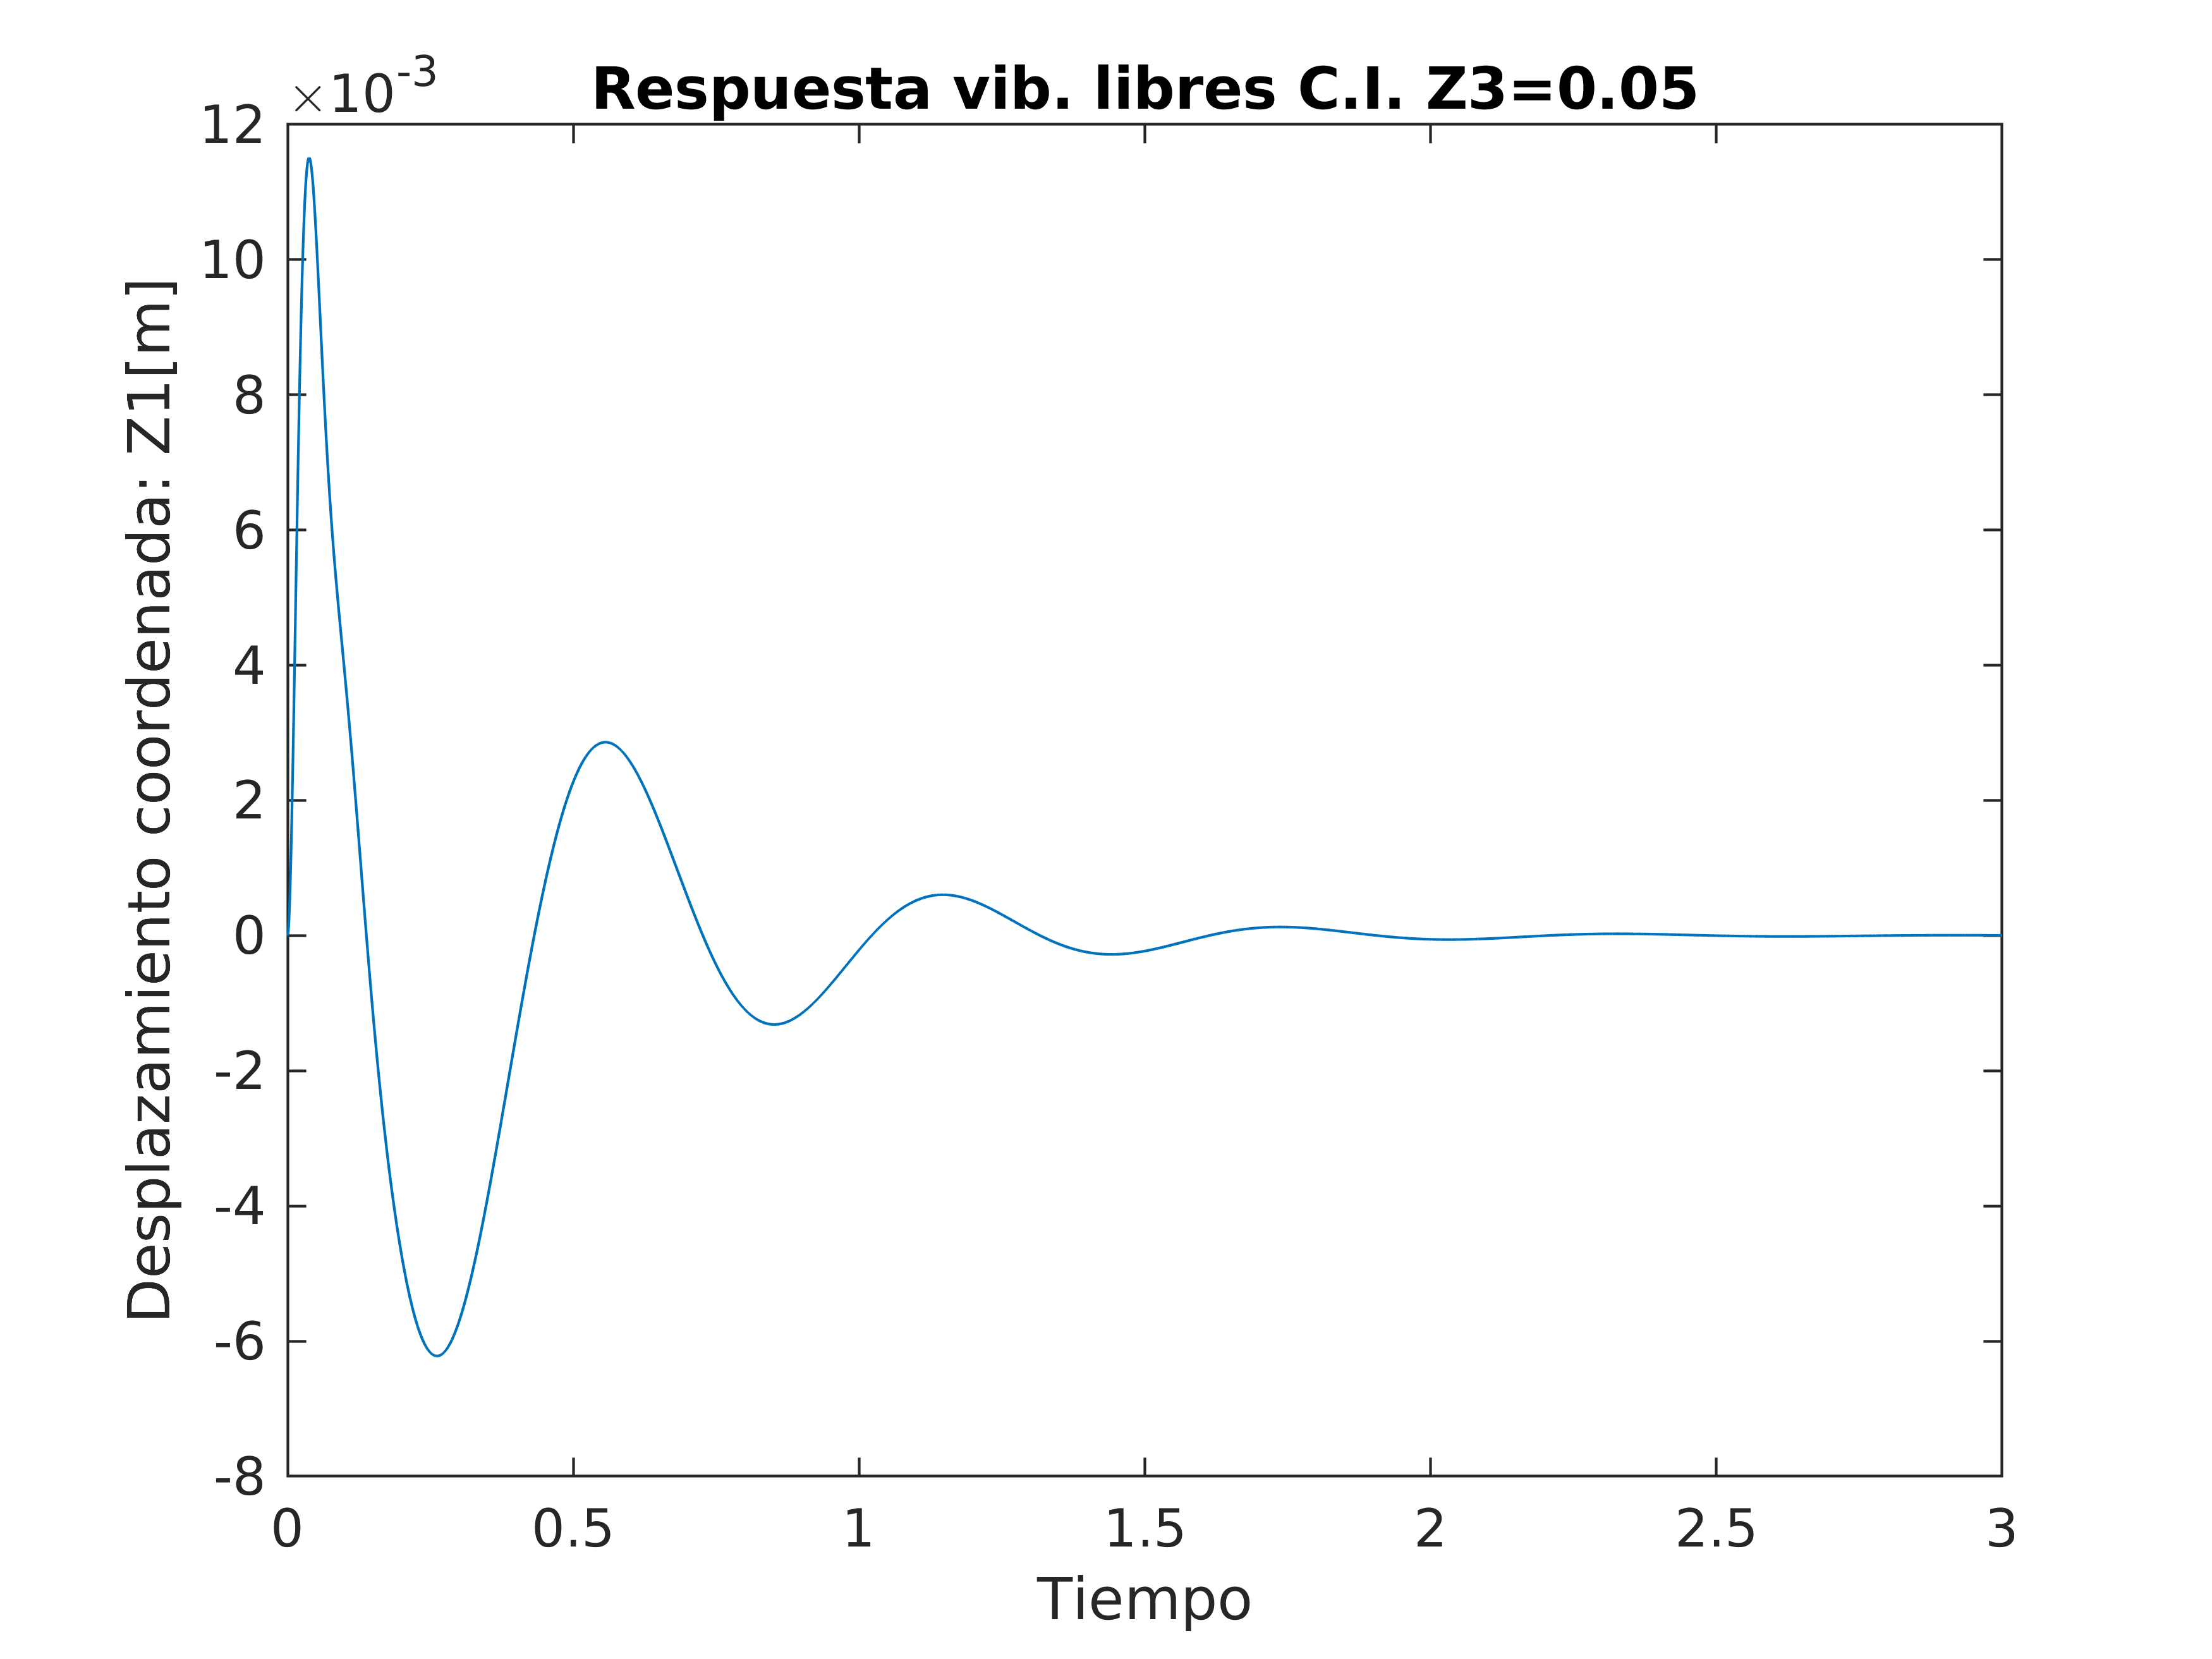
\includegraphics[width=\textwidth]{respvibZ1.png}
        \caption[]%
        {{\small Primer GDL}}    
    \end{subfigure}
    \hfill
    \begin{subfigure}[b]{0.475\textwidth}  
        \centering 
        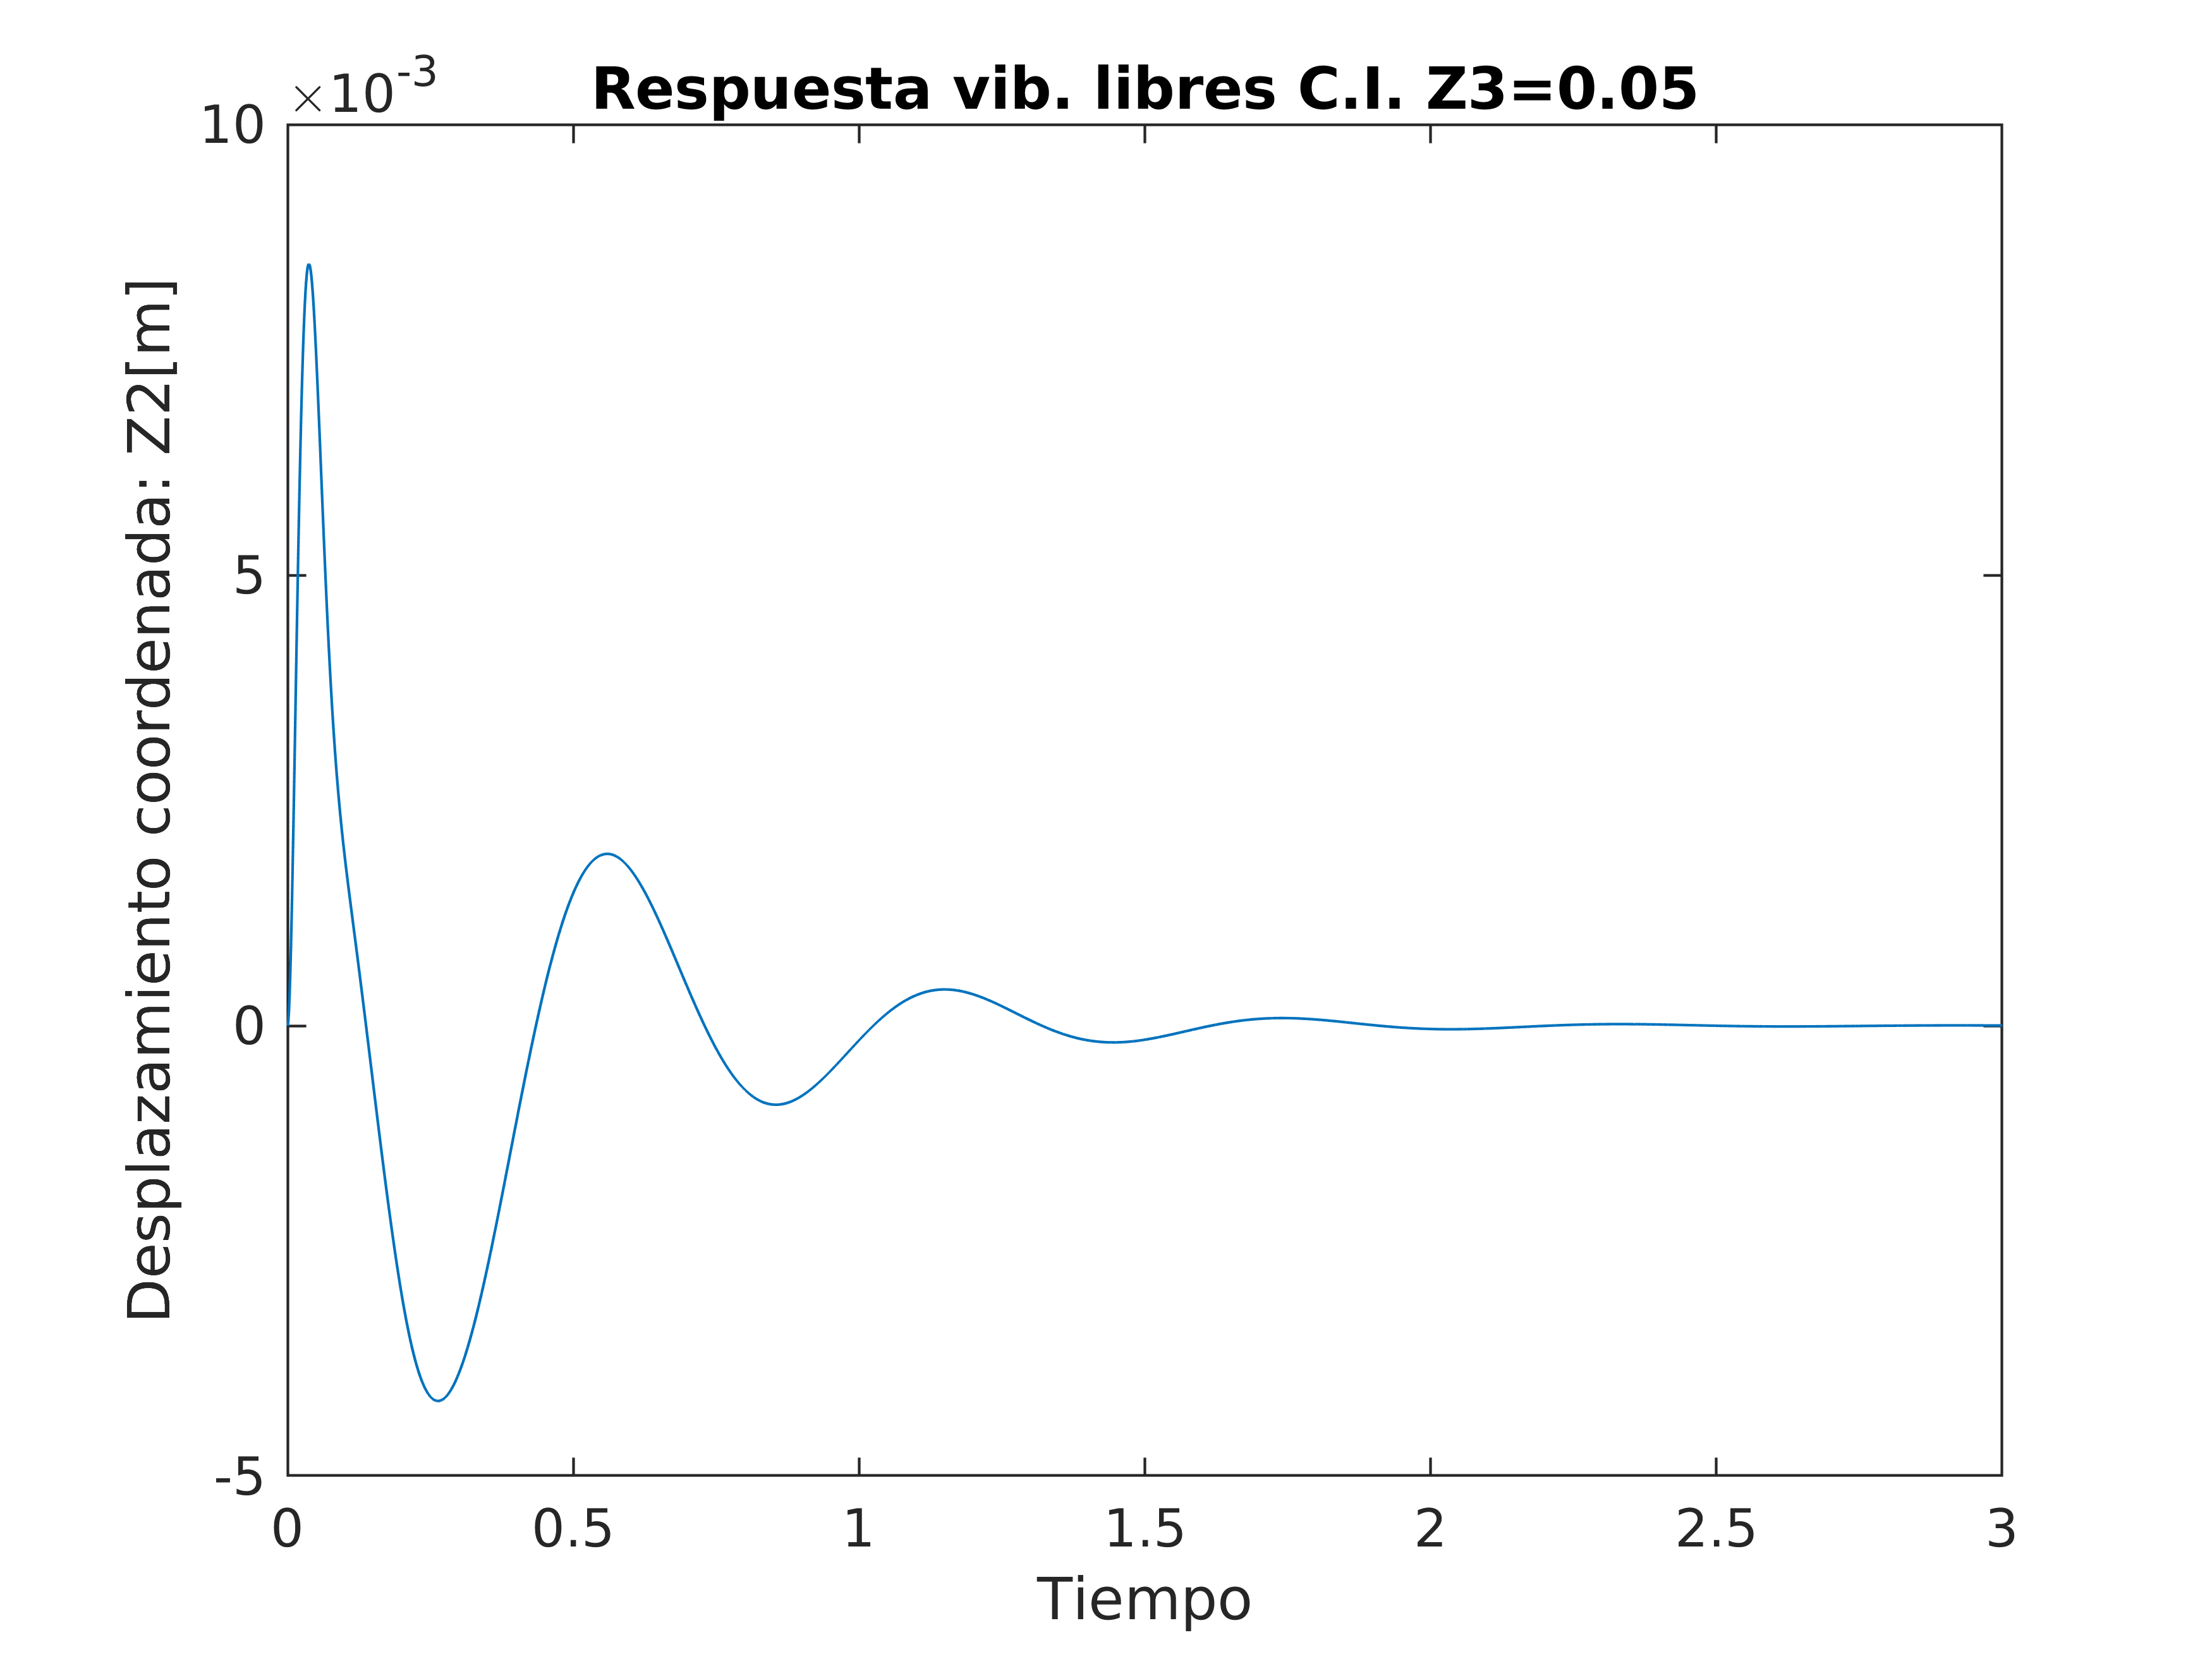
\includegraphics[width=\textwidth]{respvibZ2.png}
        \caption[]%
        {{\small Segundo GDL}}    
    \end{subfigure}
    \vskip\baselineskip
    \begin{subfigure}[b]{0.475\textwidth}   
        \centering 
        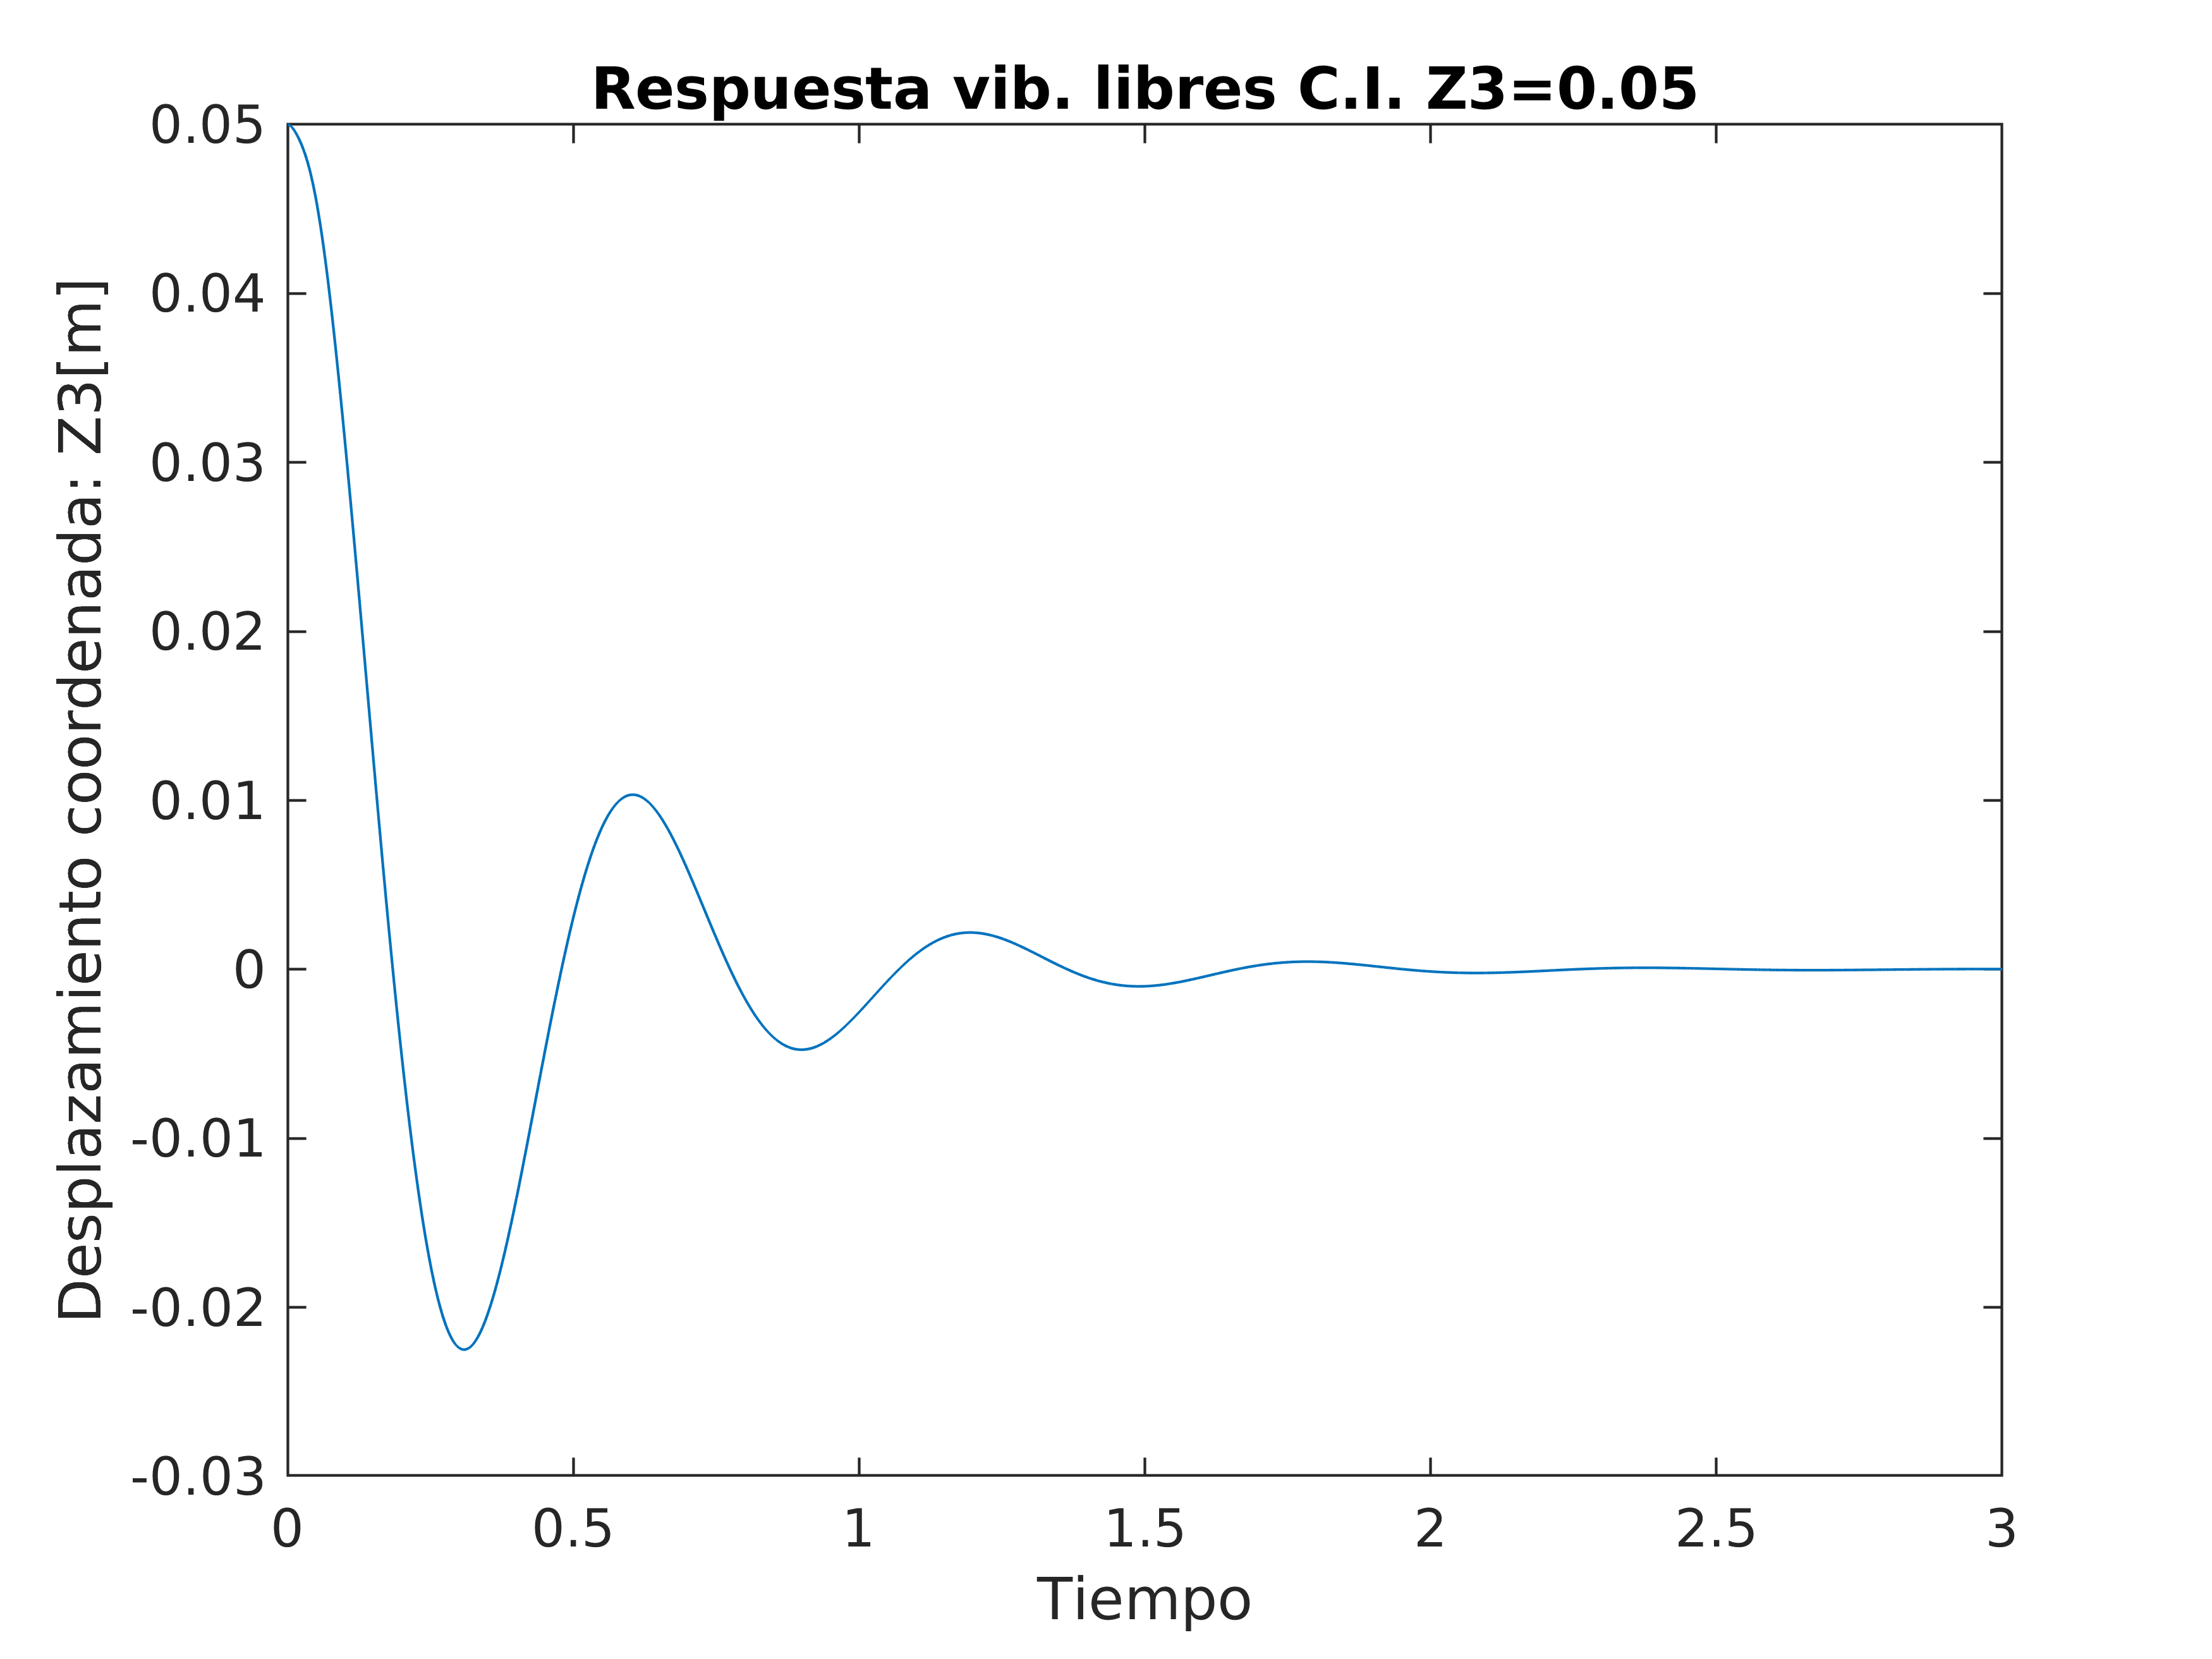
\includegraphics[width=\textwidth]{respvibZ3.png}
        \caption[]%
        {{\small Tercer GDL}}    
    \end{subfigure}
    \quad
    \begin{subfigure}[b]{0.475\textwidth}   
        \centering 
        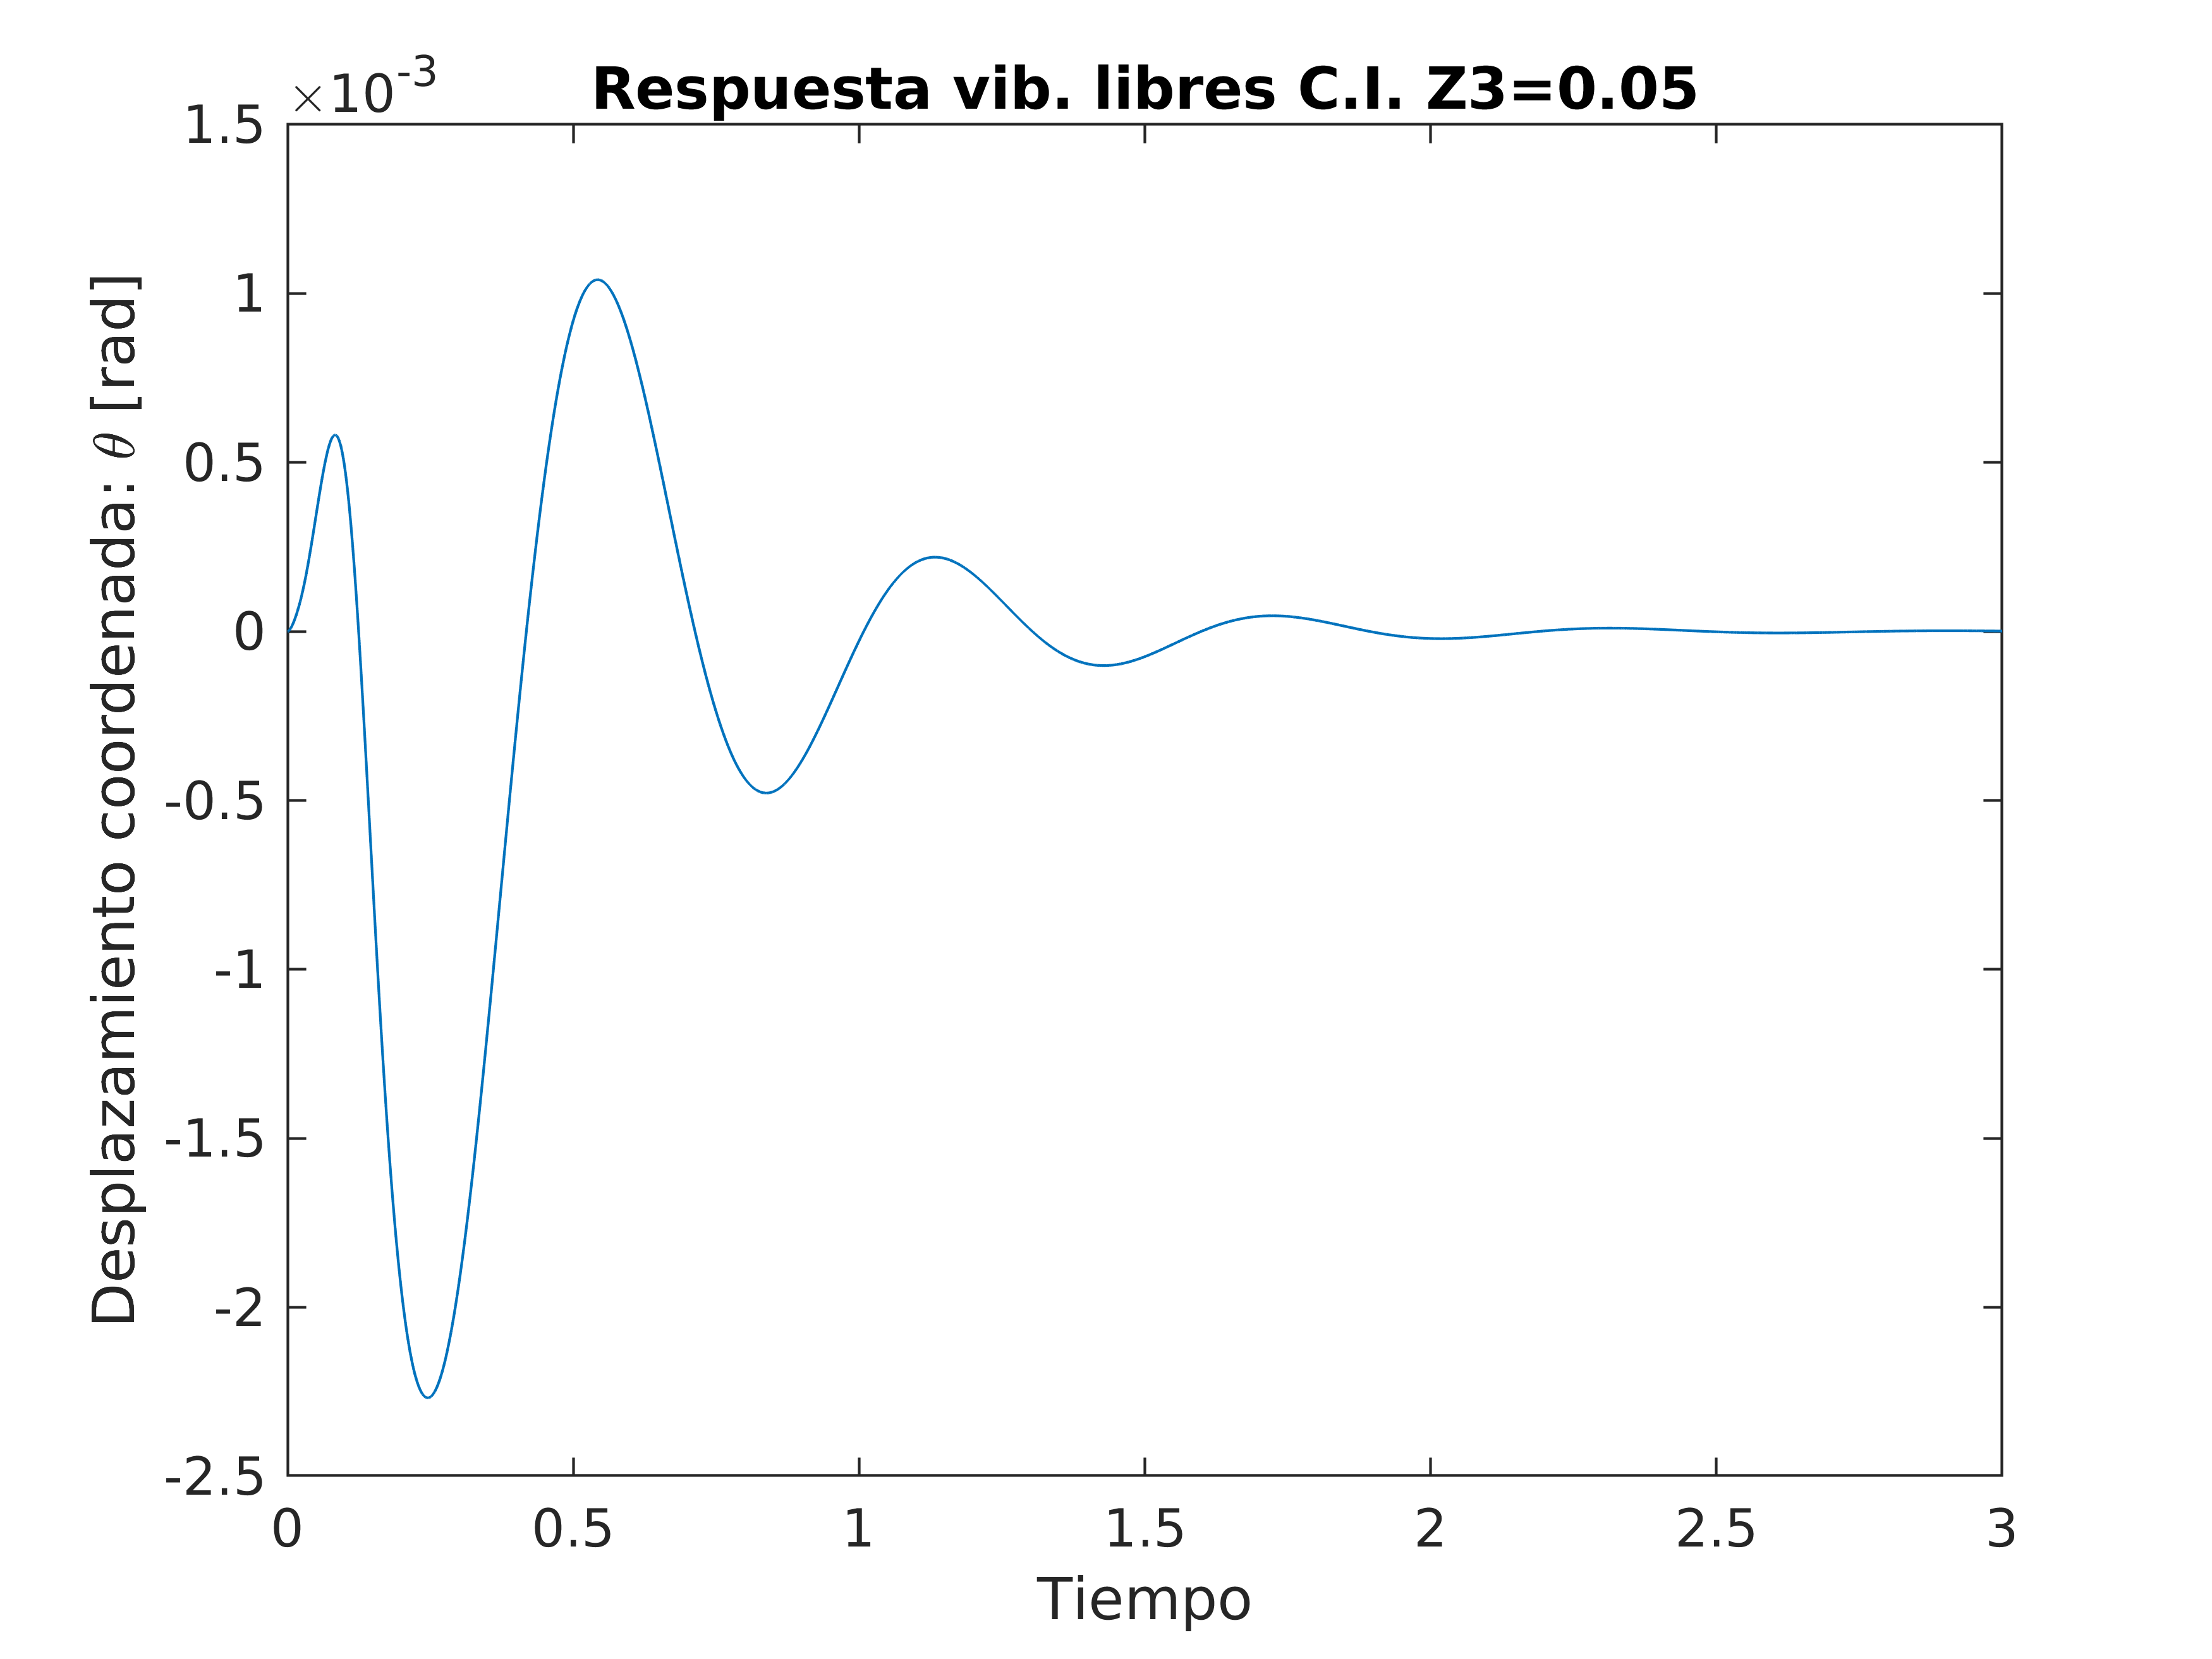
\includegraphics[width=\textwidth]{respvibtheta.png}
        \caption[]%
        {{\small Cuarto GDL}}    
    \end{subfigure}
    \caption[  ]
    {\small Respuestas para cada GDL en vibraciones libres con C.I. Z3 = 0.05} 
    \label{fig:vib lib}
\end{figure*}

\newpage
\section{Respuesta a vibraciones forzadas con carga armónica}
\label{sec: vib forz}

Esta sección está motivada por el fenómeno llamado ``serrucho`` que se puede observar en algunos caminos de tierra (ver figura \ref{fig:serrucho}). Se calculó la respuesta del sistema a este tipo de carga, con el vehículo a distintas velocidades. La velocidad del vehículo genera una variación de la frecuencia de la carga así como en las amplitudes y las relaciones entre los distintos grados de libertad.

\begin{figure}[h]
    \centering
    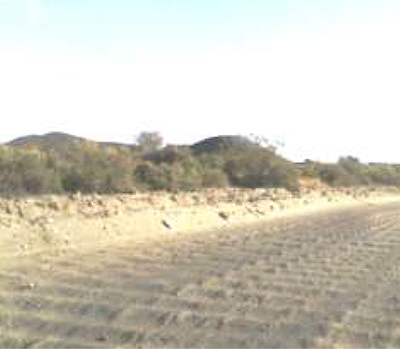
\includegraphics[width=0.5\textwidth]{serruchos.jpg}
    \caption{Serrucho en camino de tierra}
    \label{fig:serrucho}
\end{figure}

\subsection{Caracterización de la carga}

Para modelar el ``serrucho`` utilizamos una función senoidal con una amplitud de 4 cm y una longitud de onda de 35 cm, valores típicos para una onda de este estilo. La frecuencia en la que se aplica la carga es proporcional a la velocidad del automóvil.

\begin{lstlisting}
% Descripcion de la carga
A = 0.04;
lambda = 0.35;

% Velocidades
v = [5 20 60 100];
wl = 2*pi*v/lambda;     % frec de la carga, funcion de la vel del auto

\end{lstlisting}

Los grados de libertad afectados por la carga son $z_1$ y $z_2$. Debido a la distancia que separa los puntos de aplicación de la carga en el auto, existe un ángulo de fase entre $zg_1$ y $zg_2$

\begin{lstlisting}
phase = (((l1 + l2)/lambda) - floor((l1 + l2)/lambda))*2*pi;
\end{lstlisting}{}

\subsection{Respuesta}
\label{sec: resp a vib forz arm}

Para poder calcular la respuesta del sistema, nuevamente hicimos uso de la función \textit{ode45} con la subrutina especificada en la sección \ref{sec:ode45}. 

Con una velocidad de 60km/h, la respuesta es la que se observa en la figura \ref{fig:vib forz vel 60}. 

Al momento de realizar el modelado, se decidió que los grados de libertad \textit{$z_1$} y \textit{$z_2$} estén referenciados a la línea de cero de la carga externa. Sin embargo para poder comparar las respuestas a distintas velocidades y para poder visualizar más claramente los datos se decidió no imprimir los valores de los desplazamientos ``crudos`` como se obtienen del \textit{ode45} sino los desplazamientos \textit{relativos} de cada una de las ruedas al soporte. Entonces, lo que se ve en los gráficos es, de forma genérica para \textit{$z_1$} y \textit{$z_2$}: $z_{rel_i} = z_i - zg_i$.

\begin{figure*}[h]
    \centering
    \begin{subfigure}[b]{0.475\textwidth}
        \centering
        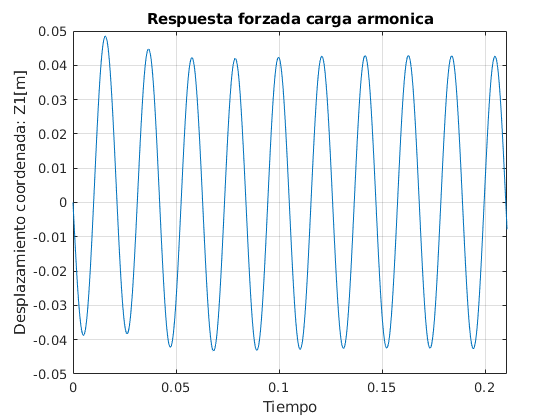
\includegraphics[width=\textwidth]{respforcompletaZ160kmh.png}
        \caption[]%
        {{\small Primer GDL}}    
    \end{subfigure}
    \hfill
    \begin{subfigure}[b]{0.475\textwidth}  
        \centering 
        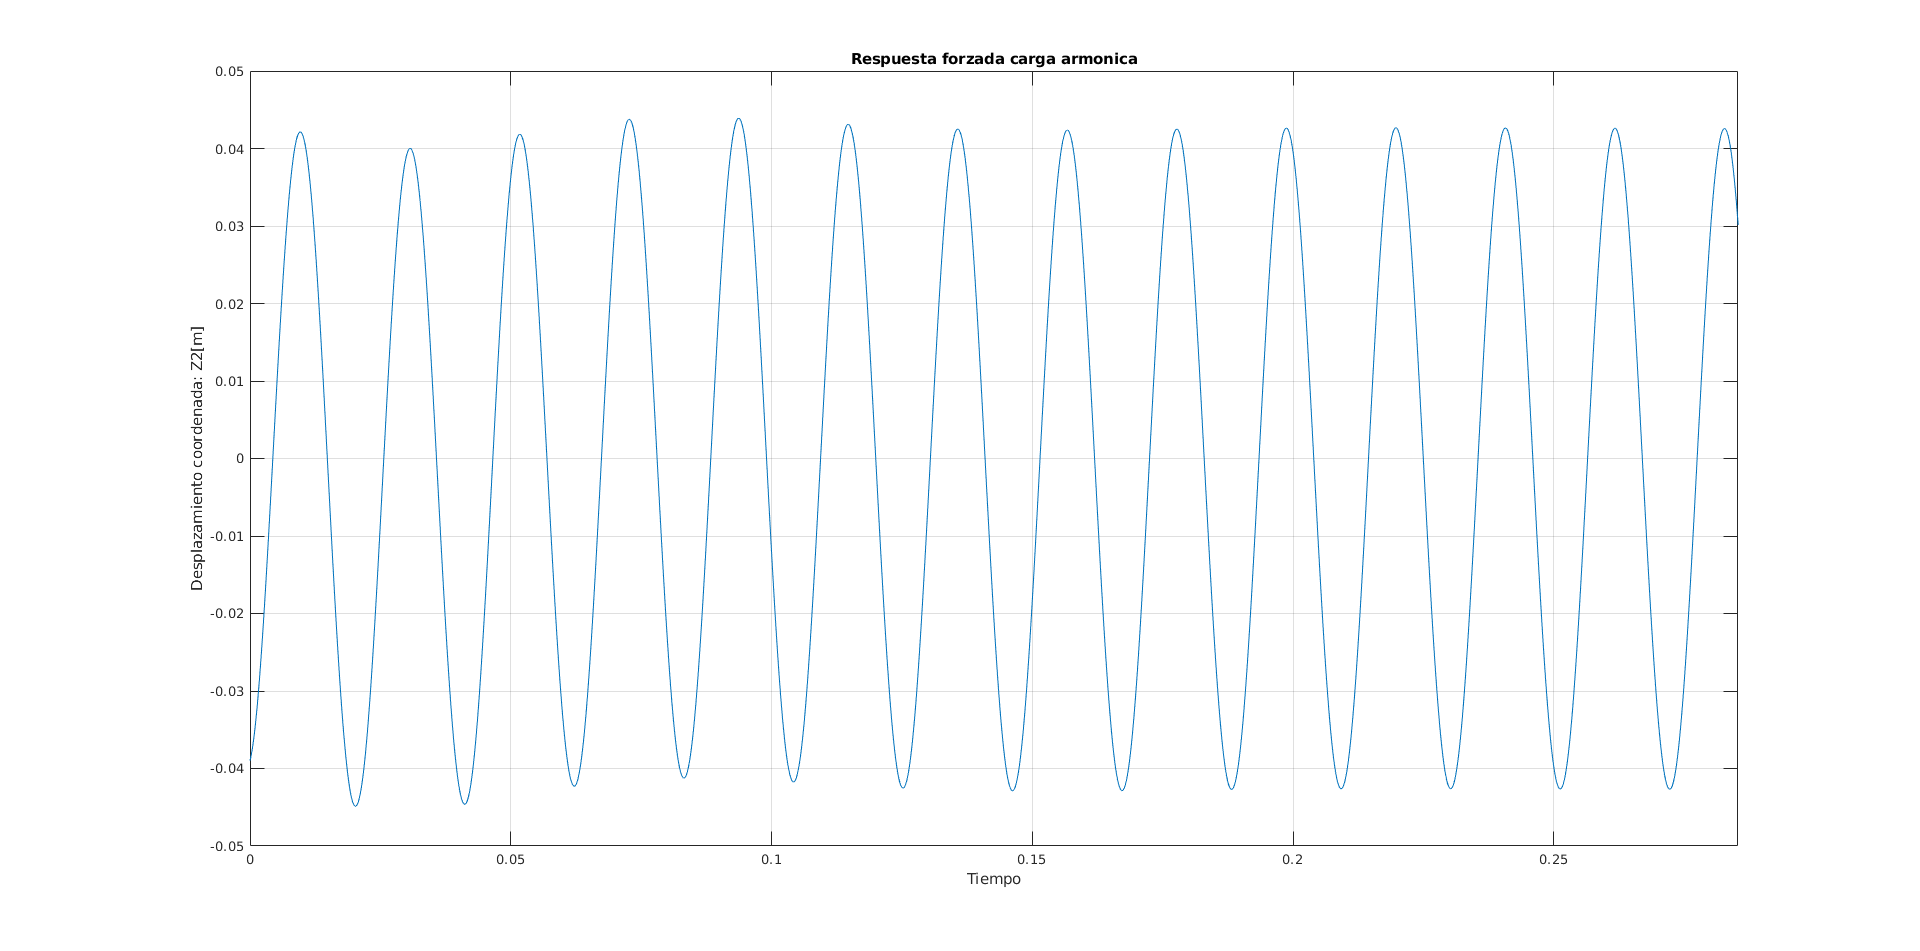
\includegraphics[width=\textwidth]{respforcompletaZ260kmh.png}
        \caption[]%
        {{\small Segundo GDL}}    
    \end{subfigure}
    \vskip\baselineskip
    \begin{subfigure}[b]{0.475\textwidth}   
        \centering 
        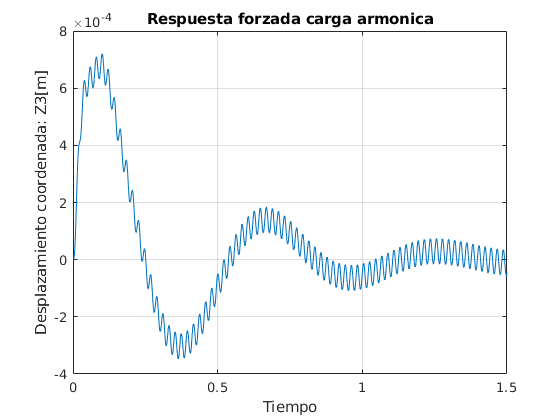
\includegraphics[width=\textwidth]{respforcompletaZ360kmh.png}
        \caption[]%
        {{\small Tercer GDL}}    
    \end{subfigure}
    \quad
    \begin{subfigure}[b]{0.475\textwidth}   
        \centering 
        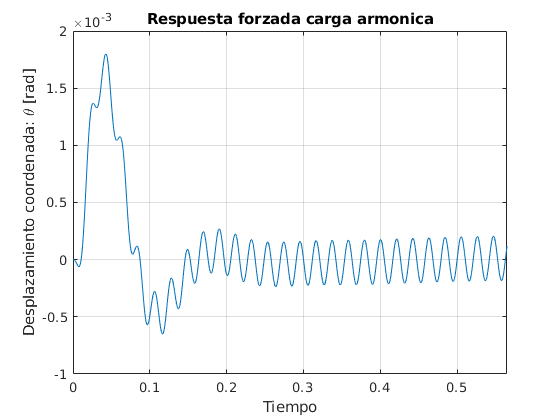
\includegraphics[width=\textwidth]{respforcompletatheta60kmh.png}
        \caption[]%
        {{\small Cuarto GDL}}    
    \end{subfigure}
    \caption[  ]
    {\small Respuestas para cada GDL para una velocidad de 60 km/h} 
    \label{fig:vib forz vel 60}
\end{figure*}

\newpage
\subsubsection{Comparación de las respuestas a distintas velocidades}

Se comparan las respuestas dadas en $z_1$ y $z_3$ (una rueda y el chasis). 
Para $z_1$ las respuestas a distintas velocidades son la de la figura \ref{fig:z1 vib forz}.

\begin{figure*}[h]
    \centering
    \begin{subfigure}[b]{0.475\textwidth}
        \centering
        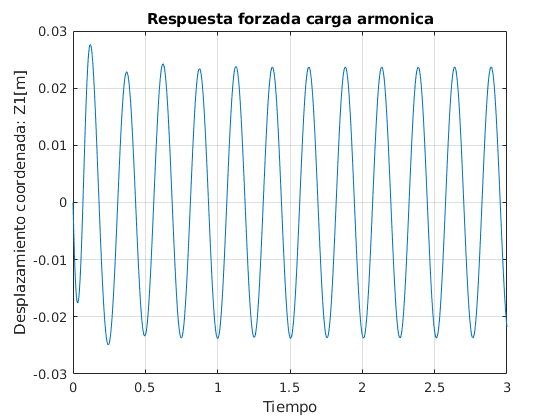
\includegraphics[width=\textwidth]{respforcompletaZ15kmh.png}
        \caption[]
        {{\small Primer GDL a 5km/h}}    
    \end{subfigure}
    \hfill
    \begin{subfigure}[b]{0.475\textwidth}  
        \centering 
        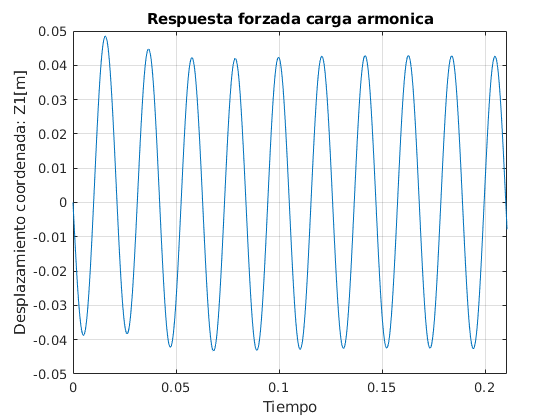
\includegraphics[width=\textwidth]{respforcompletaZ160kmh.png}
        \caption[]
        {{\small Primer GDL a 60km/h}}    
    \end{subfigure}
    \vskip\baselineskip
    \begin{subfigure}[b]{0.475\textwidth}   
        \centering 
        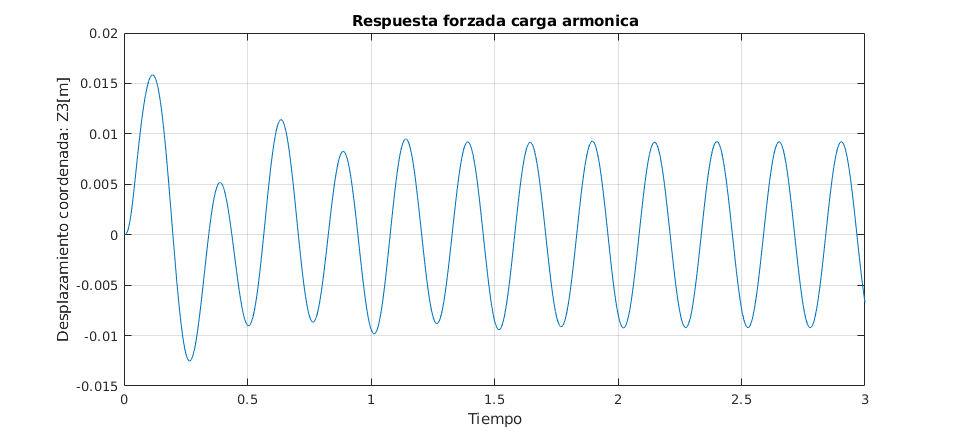
\includegraphics[width=\textwidth]{respforcompletaZ35kmh.png}
        \caption[]
        {{\small Tercer GDL a 5 km/h}}    
    \end{subfigure}
    \quad
    \begin{subfigure}[b]{0.475\textwidth}   
        \centering 
        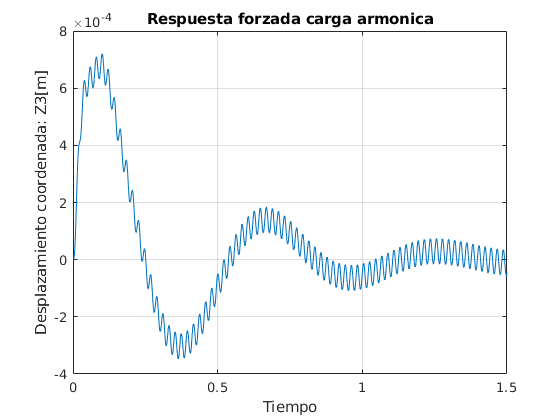
\includegraphics[width=\textwidth]{respforcompletaZ360kmh.png}
        \caption[]
        {{\small Tercer GDL a 60 km/h}}    

    \end{subfigure}
    \caption[  ]
    {\small Respuestas para $z_1$ y $z_3$ para distintas velocidades} 
    \label{fig:z1 vib forz}
\end{figure*}

Observamos que a mayores velocidades del vehículo la frecuencia forzada es mayor y las amplitudes de $z_3$ disminuyen. Además, se observa que esta disminución de la amplitud se ve ``absorbida`` por los movimientos de $z_1$ y $z_2$. 

\newpage
\section{Respuesta a carga impulsiva}

En esta sección se desea encontrar la respuesta del sistema a una carga impulsiva. Dicha carga podría ser obtenida al, por ejemplo, pasar por un ``lomo de burro``.

\subsection{Descripción de la carga}
La carga en sí fue modelada como una carga triangular con una altura de $0,1$ m y $0,2$ m de ancho. Se calculó la respuesta del sistema a esta carga, con el vehículo a distintas velocidades. 

Los grados de libertad \textit{$z_1$} y \textit{$z_2$} son afectados por distintas cargas ya que hay un desfasaje entre el momento en el que el primer y el segundo grado de libertad se ven excitados. Esto se observa en la figura \ref{fig: impulso dist velocidades}, donde a mayores velocidades, menor es el espaciamiento temporal entre los dos picos.

\begin{figure*}[h]
    \centering
    \begin{subfigure}[b]{0.475\textwidth}
        \centering
        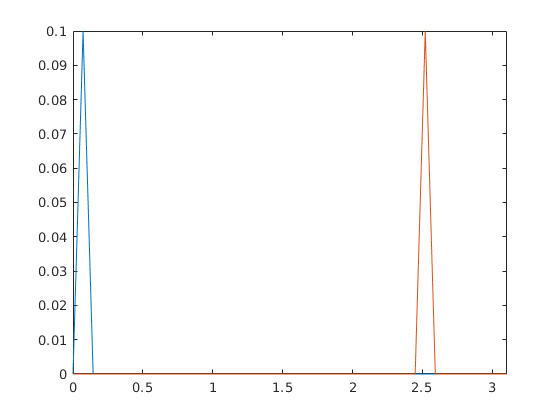
\includegraphics[width=\textwidth]{picos5kmh.png}
        \caption[]%
        {{\small A 5 km/h}}    
    \end{subfigure}
    \hfill
    \begin{subfigure}[b]{0.475\textwidth}  
        \centering 
        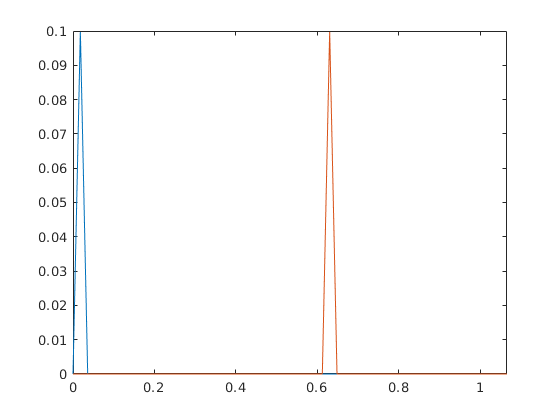
\includegraphics[width=\textwidth]{picos20kmh.png}
        \caption[]%
        {{\small A 20 km/h}}    
    \end{subfigure}
    \vskip\baselineskip
    \begin{subfigure}[b]{0.475\textwidth}   
        \centering 
        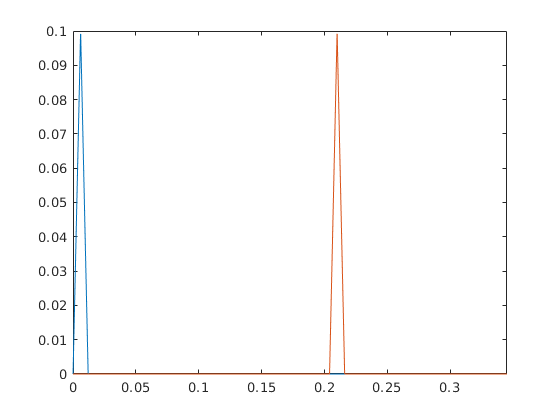
\includegraphics[width=\textwidth]{picos60kmh.png}
        \caption[]%
        {{\small A 60 km/h}}    
    \end{subfigure}
    \quad
    \begin{subfigure}[b]{0.475\textwidth}   
        \centering 
        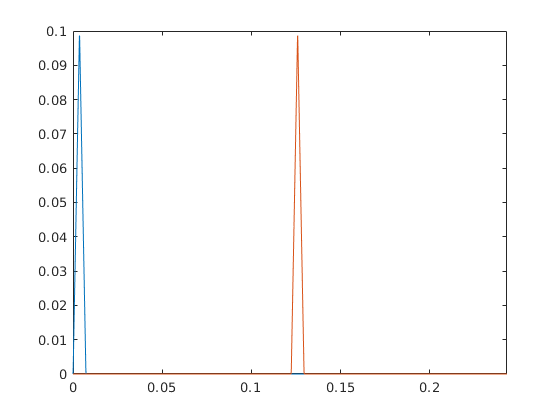
\includegraphics[width=\textwidth]{picos100kmh.png}
        \caption[]%
        {{\small A 100 km/h}}    
    \end{subfigure}
    \caption[  ]
    {\small Carga impulsiva a distintas velocidades. En azul para $z_1$ y en rojo para $z_2$. Las cargas externas para los otros grados de libertad son cero} 
    \label{fig: impulso dist velocidades}
\end{figure*}

\subsection{Respuesta}

Para obtener la respuesta a dichas cargas impulsivas se utilizó el método de diferencia central tal como se explicó en la sección \ref{sec:dif finitas}. 

Cada grado de libertad producirá distintas respuestas para las cargas dadas en la figura \ref{fig: impulso dist velocidades}; se muestran las respuestas para \textit{${z_1}$} y \textit{$ {z_3}$} en la figura \ref{fig: resp z1 impulso dist velocidades}.

Además se compararon las respuestas de todos los grados de libertad; se pueden observar las respuestas a 20 km/h, por ejemplo, en la figura \ref{fig: resp 4gdl impulso dist velocidades} y comparar los grados de libertad correspondientes con los mostrados en la figura \ref{fig: resp z1 impulso dist velocidades}.

Así como se explicó en la sección \ref{sec: resp a vib forz arm}, los resultados de los gráficos para los primeros dos GDL son las amplitudes \textit{relativas} de las ruedas al soporte, por las mismas razones ya explicadas.  

\Floatbarrier
\begin{figure*}[h]
    \centering
    \begin{subfigure}[b]{0.475\textwidth}
        \centering
        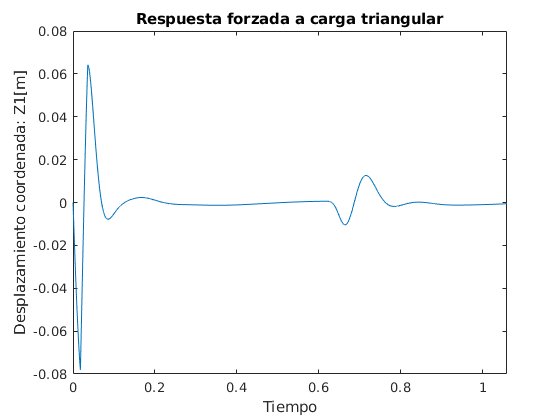
\includegraphics[width=\textwidth]{difcent,picos,Z120kmh.png}
        \caption[]%
        {{\small Primer GDL}}    
    \end{subfigure}
    \hfill
    \begin{subfigure}[b]{0.475\textwidth}  
        \centering 
        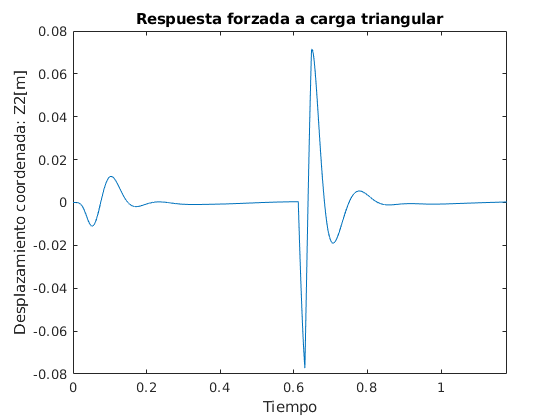
\includegraphics[width=\textwidth]{difcent,picos,Z220kmh.png}
        \caption[]%
        {{\small Segundo GDL}}    
    \end{subfigure}
    \vskip\baselineskip
    \begin{subfigure}[b]{0.475\textwidth}   
        \centering 
        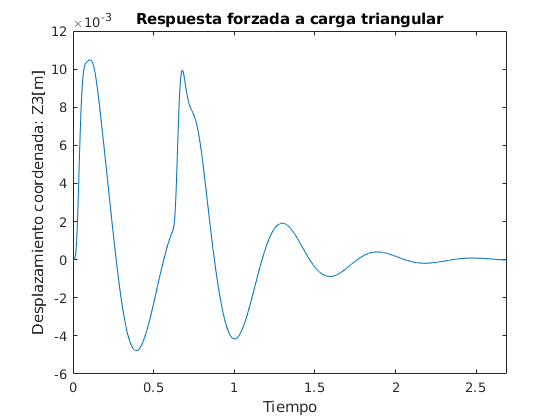
\includegraphics[width=\textwidth]{difcent,picos,Z320kmh.png}
        \caption[]%
        {{\small Tercer GDL}}    
    \end{subfigure}
    \quad
    \begin{subfigure}[b]{0.475\textwidth}   
        \centering 
        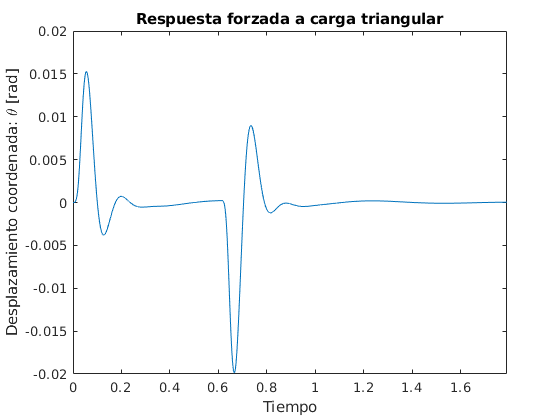
\includegraphics[width=\textwidth]{difcent,picos,theta20kmh.png}
        \caption[]%
        {{\small Cuarto GDL}}    
    \end{subfigure}
    \caption[  ]
    {\small Respuesta a carga impulsiva a distintos GDL a 20km/h} 
    \label{fig: resp 4gdl impulso dist velocidades}
\end{figure*}
\Floatbarrier

\Floatbarrier
\begin{figure*}[h]
    \centering
    \begin{subfigure}[b]{0.475\textwidth}
        \centering
        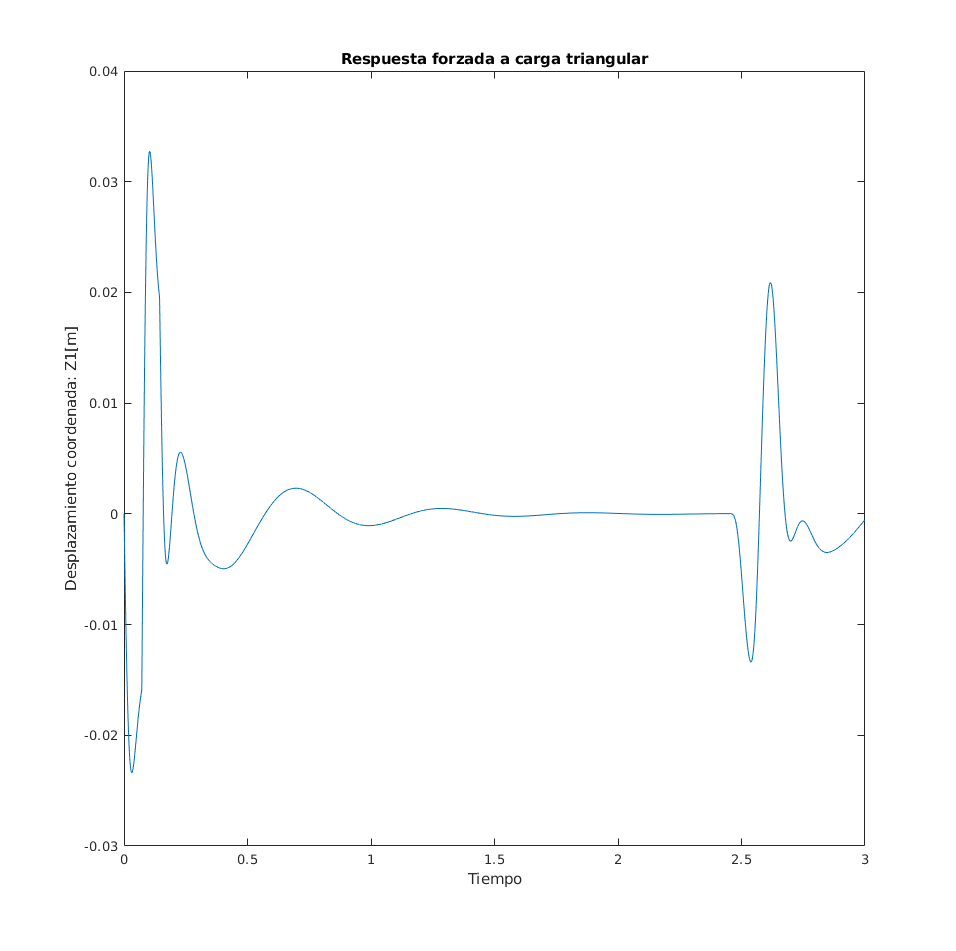
\includegraphics[width=\textwidth]{difcent,picos,Z15kmh.png}
        \caption[]%
        {{\small $z_1$ a 5 km/h}}    
    \end{subfigure}
    \hfill
    \begin{subfigure}[b]{0.475\textwidth}  
        \centering 
        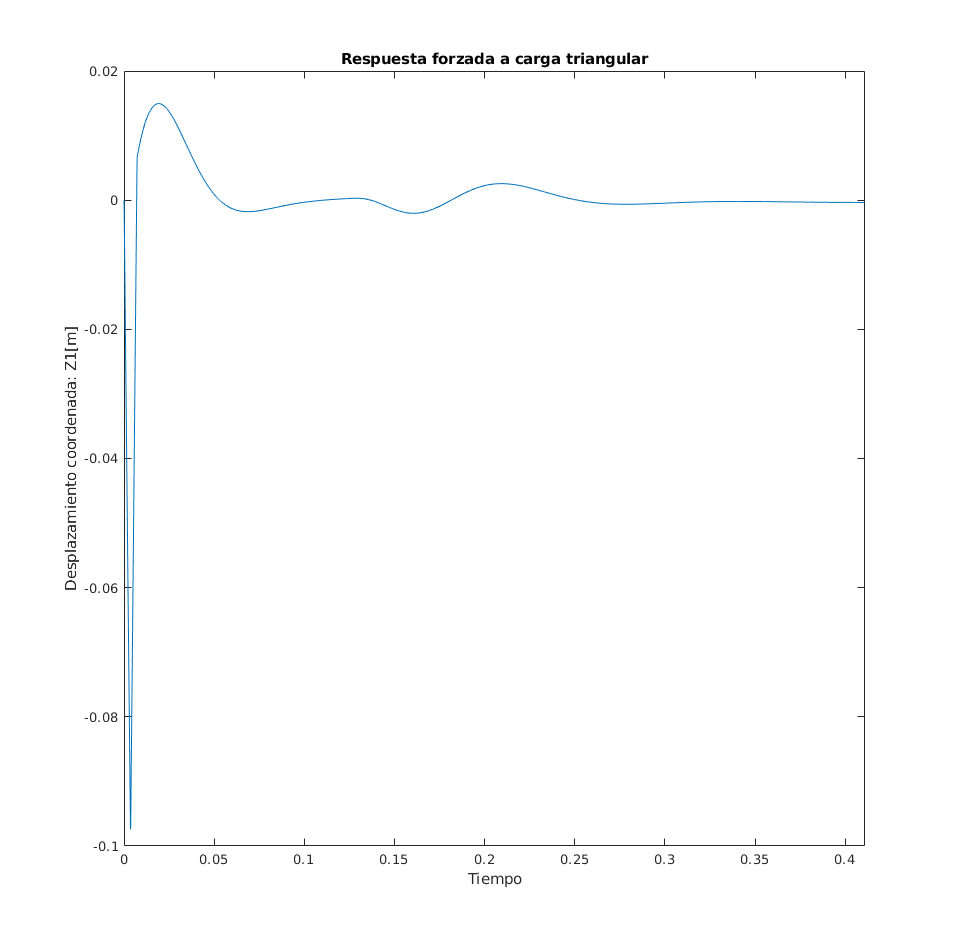
\includegraphics[width=\textwidth]{difcent,picos,Z1100kmh.png}
        \caption[]%
        {{\small $z_1$ a 100 km/h}}    
    \end{subfigure}
    \vskip\baselineskip
    \begin{subfigure}[b]{0.475\textwidth}   
        \centering 
        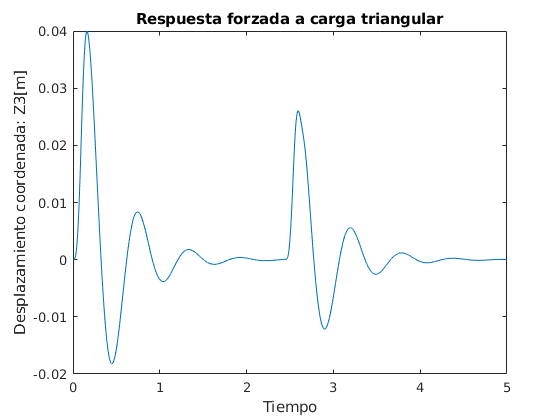
\includegraphics[width=\textwidth]{difcent,picos,Z35kmh.png}
        \caption[]%
        {{\small $z_3$ a 5 km/h}}    
    \end{subfigure}
    \quad
    \begin{subfigure}[b]{0.475\textwidth}   
        \centering 
        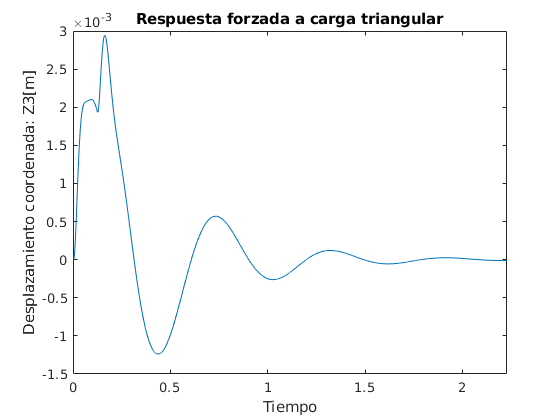
\includegraphics[width=\textwidth]{difcent,picos,Z3100kmh.png}
        \caption[]%
        {{\small $z_3$ a 100 km/h}}    
    \end{subfigure}
    \caption[  ]
    {\small Respuesta a carga impulsiva a distintas velocidades para $z_1$ y $z_3$} 
    \label{fig: resp z1 impulso dist velocidades}
\end{figure*}

\Floatbarrier

Podemos observar que a mayores velocidades la amplitud de la respuesta para \textit{$z_3$} es cada vez menor, mientras que aumentan las amplitudes de los grados de libertad \textit{$z_1$} y \textit{$z_2$}. De esta forma podemos concluir que yendo a mayores velocidades ``sufre`` más el sistema de amortiguación y la cubierta pero la amplitud del movimiento que notaría el pasajero es menor. Lo contrario sucede a velocidades bajas: grandes amplitudes en el chasis pero pequeñas en los primeros dos grados de libertad.

\newpage
\section{Discusión y conclusiones}
A través de este trabajo se han llegado a varias conclusiones, una de ellas es que para una carga impulsiva dada, la velocidad de vehículo es importante para la determinación de la amplitud de las respuestas. A velocidades bajas la respuesta (en amplitud) del chasis será alta y la del neumático baja, en cambio, para velocidades altas, la amplitud de la respuesta de los neumáticos será mucho mayor a la del chasis.

Para cargas armónicas observamos el mismo fenómeno que para la carga impulsiva: a velocidades bajas la amplitud de respuesta para \textit{$z_3$} son mayores y esta va disminuyendo a medida que aumenta la velocidad; caso contrario ocurre con \textit{$z_1$} y \textit{$z_2$} que a medida que aumenta la velocidad aumenta la amplitud de su respuesta. Esto se puede traducir en que a bajas velocidades, el pasajero siente más el impacto del sistema de amortiguamiento, en cambio a velocidades altas no la siente tanto pero la fuerza sobre el sistema de amortiguamiento del vehículo y sobre los neumáticos aumenta.

%\printbibliography
% \bibliography{biblioteca}
\section{Referencias}



Hurel Ezeta, Jorge L. Modelado analítico y control inteligente de un sistema de suspensión activa para un cuarto de vehículo. Tesis doctoral. Universidad de Málaga. 2013


Goulart Campos; Caldeira; Norohna de Oliveira; Peralta Y Da Costa Neto. Suspension parameters estimation of a RWD vehicle. SAE Technical paper series. 2017



Peralta, Alejandro; Heidenreich,Elvio ; Caldeira,  Aldélio y Neto, Ricardo.Estimación de los parámetros equivalentes de la suspensión de un vehículo pesado 6 x 6. CAIM. 2018

TICA Mihai, DOBRE George et al. Optimal damping constant of the quarter car shock absorber. 2012 \label{libro_tabla}



\newpage
\tableofcontents
\end{document}



